\documentclass[12pt, a4paper]{report} 
\usepackage{graphicx}
\graphicspath{ {./images/} }
\usepackage[a4paper, margin=1in]{geometry}
\usepackage{fontspec}
% \usepackage{biblatex} %Imports biblatex package
% \addbibresource{references.bib} %Import the bibliography file
\setmainfont{Times New Roman}

% Load any additional packages
\usepackage{array}
\usepackage{amssymb}
\usepackage{amsmath}
\usepackage{natbib}
\usepackage{multicol}
\usepackage{xcolor}
%\usepackage{helvet}
%\renewcommand{\familydefault}{\sfdefault}
\usepackage{acronym} 
\usepackage{nomencl}
\usepackage{array}
\usepackage{subfig}
\usepackage{algorithm}
\usepackage{algpseudocode}
\usepackage[justification=centering]{caption}
\usepackage{enumitem}
%\usepackage{hyperref} for hyperlink
\usepackage{tabulary}
\usepackage[document]{ragged2e}
\usepackage{svg}
\usepackage{cite}
\usepackage{ragged2e}
\usepackage{indentfirst}
\usepackage{subfiles}
\usepackage{titlesec}
\usepackage{hyperref}

\hypersetup{
    colorlinks=true, 
    linkcolor=black, 
    urlcolor=black, 
    citecolor=black, 
    pdfauthor=Niranjan Jadhav, 
    pdftitle={BTech\_Project\_Report\_2024-25}
}

% \titleformat{\chapter}[block]{\LARGE\bfseries}{\thechapter.}{0.5em}{}
% \titlespacing*{\chapter}{0pt}{10pt}{5pt}

% \titleformat{\section}[block]{\Large\bfseries}{\thesection}{0.5em}{}
% \titlespacing{\section}{0pt}{5pt}{5pt}

% \titleformat{\subsection}[block]{\large\bfseries}{\thesubsection}{0.5em}{}
% \titlespacing{\subsection}{0pt}{5pt}{5pt}

\def\mytitle{Hardware Accelerator for Thyroid Nodule Classification}
\def\firstname{Tanvi Deshmukh}
\def\firstroll{112107013}
\def\secondname{Karan Doshi}
\def\secondroll{112107015}
\def\thirdname{Niranjan Jadhav}
\def\thirdroll{112107022}

\def\mydegree{Bachelor of Technology}
\def\mySpecialization{Electronics and Telecommunication}
\def\mysupervisor{Dr. Vaishali V. Ingale}

\def\mymonth{May}
\def\myyear{2025}

\renewcommand*\contentsname{Table of Contents}
\makenomenclature
\renewcommand{\nomname}{List of Symbols}


\begin{document}
 \baselineskip=18pt plus1pt
 \setcounter{secnumdepth}{3}
 \setcounter{tocdepth}{3}
 \pagenumbering{roman}
 
 %Front Matter %%Edit to add or remove a page/section of front matter
 \thispagestyle{empty}
\begin{center}
    { \LARGE {\bfseries {\mytitle}} \par}
\vspace{\baselineskip}
    {A Project Report \par}
    \vspace{\baselineskip}
    {\textit{Submitted in partial fulfillment for the}\\
    \textit{award of the degree of}}\par

    \vspace{\baselineskip}
    {\large {\bf {\mydegree}} \par
    \textit{in} \\
    \large \bf \mySpecialization \par}
\vspace{\baselineskip}
{\textit{by} \par}
\vspace{\baselineskip}

\begin{center}
\begin{tabular}{cl}
{\large \bf \firstroll} & {\large \bf \firstname} \\
{\large \bf \secondroll} & {\large \bf \secondname} \\
{\large \bf \thirdroll} & {\large \bf \thirdname} \\
\end{tabular}
\end{center}

%\vspace{-0.1\baselineskip}
%    {{\large {\bf \myrollno}} \par}
\vspace{1.5\baselineskip}
    {Under the guidance of \par}
\vspace{\baselineskip}
    {{\large \bf \mysupervisor} \par}
\vspace{1\baselineskip}
    {\begin{figure}[!h] 
	\centering
	
\includegraphics[width=50mm]{./images/coep_logo.jpg} 
     \end{figure}
    }
%{\large \vspace*{1ex}

\vspace*{1ex}
    {\bf Department of Electronics  and Telecommunication Engineering \par}
    {\bf COEP Technological University, Pune \par}
    {\bf (Formerly College of Engineering, Pune) \par}
    {\bf Shivajinagar, Pune-411005, Maharashtra \par}
    {\bf May-2025}
    
 \end{center}
 \newpage
 \thispagestyle{empty}

\cleardoublepage 
\vspace*{1cm}  
\phantomsection
\addcontentsline{toc}{chapter}{Certificate}
\begin{center}
{\Large {\bf \uppercase{Certificate}}}
\end{center}


\begin{figure}[H]
    \centering
    
\includegraphics[width=50mm]{images/coep_logo.jpg}
    \label{fig:certificate_logo}
\end{figure}

\vspace{\baselineskip}

\begin{justify}
\noindent This is to certify that the project report entitled {"\mytitle"}, is the bonafide work {\firstname} {(\textit \firstroll}) { \secondname} {(\textit \secondroll}) {\thirdname} {(\textit \thirdroll}) who carried out their work under my supervision. Certified to the best of my knowledge, the work reported herein does not form part of any other thesis or dissertation based on which a degree or award was conferred on an earlier occasion on this or any other candidate. 
\end{justify}
\vspace{5\baselineskip}
\begin{center}
    \begin{minipage}[c]{0.45\textwidth}
        \centering
        \hrule 
        \vspace{0.5\baselineskip}
        \flushleft{{\large \bf Project Guide} \\
        {Dr. Vaishali Ingale} \\
        {Department of Electronics \& Telecommunication} \\
        COEP Technological University, Pune}
    \end{minipage}
    \hfill % Adds space between the two mini pages
    \begin{minipage}[c]{0.45\textwidth}
        \centering
        \hrule 
        \vspace{0.5\baselineskip}
        \flushleft{{\large \bf Head of Department} \\
        {Dr. Vibha Vyas} \\
        {Department of Electronics \& Telecommunication} \\
        COEP Technological University, Pune}
    \end{minipage}
\end{center}

\vspace{3\baselineskip}
\noindent
COEP Technological University, Pune \\
Date: 10 May 2025


 \thispagestyle{empty}

\cleardoublepage 
\vspace*{1cm}  
\phantomsection
\addcontentsline{toc}{chapter}{Approval Sheet}
\begin{center}
    \textbf{\Large APPROVAL SHEET}
    \vspace{1.5\baselineskip}

    \large This report entitled,
    \vspace{\baselineskip}

    \textbf{\Large Hardware Accelerator for Thyroid Nodule
Classification}
    \vspace{\baselineskip}

    \textit{submitted by,} 
    \vspace{\baselineskip}

    \textbf{112107013 - Tanvi Deshmukh} \\
    \textbf{112107015 - Karan Doshi} \\
    \textbf{112107022 - Niranjan Jadhav}
    \vspace{\baselineskip}

    is approved for the degree of
    \vspace{\baselineskip}

    \textbf{Bachelor of Technology} \par
    \vspace{0.5\baselineskip}
    \textit{in} \par
    \vspace{0.5\baselineskip}
    \textbf{Department of Electronics and Telecommunication Engineering}
    \vspace{\baselineskip}

    \textbf{COEP Technological University, Pune} \\
    \textbf{(A Unitary Public University of Government of Maharashtra)}
\end{center}

\vspace{2\baselineskip}

\begin{center}
\large
\begin{tabular}{lll}
\textbf{Examiners} & \textbf{Name} & \textbf{Signature} \\[1em]
1. External Examiner & \rule{5cm}{0.4pt} & \rule{4cm}{0.4pt} \\[1em]
2. Internal Examiner & \rule{5cm}{0.4pt} & \rule{4cm}{0.4pt} \\[1em]
3. HOD & \rule{5cm}{0.4pt} & \rule{4cm}{0.4pt} \\
\end{tabular}
\end{center}

\vspace{2\baselineskip}

Date: 10 May 2025\\
Place: Pune



 \newpage
 \thispagestyle{empty}

\cleardoublepage 
\vspace*{1cm}  
\phantomsection
\addcontentsline{toc}{chapter}{Declaration}
\begin{center}
 \Large {\bf \uppercase{Declaration}}
\end{center}

\vspace{2\baselineskip}
\begin{justify}
\noindent
We declare that this written submission represents our ideas in our own words, and where others' ideas or words have been included, we have adequately cited and referenced the sources. We also declare that we have adhered to all principles of academic honesty and integrity and have not misrepresented or fabricated, or falsified any idea/data/fact/source in our submission. We understand that any violation of the above will be cause for disciplinary action by the Institute and can also evoke penal action from the sources which have thus not been properly cited or from whom proper permission has not been taken when needed.
\end{justify}

\vspace{1.5\baselineskip}

\begin{center}
\begin{tabular}{lll}
\textbf{Name} & \textbf{Roll Number} & \textbf{Signature} \\[1em]
Tanvi Anil Deshmukh & 112107013 & \rule{4cm}{0.4pt} \\[1em]
Karan Rajkumar Doshi & 112107015 & \rule{4cm}{0.4pt} \\[1em]
Niranjan Pratapsinh Jadhav & 112107022 & \rule{4cm}{0.4pt} \\
\end{tabular}
\end{center}


\vspace{4\baselineskip}
\noindent
COEP Technological University, Pune \\
Date: 10 May 2025


 
 \thispagestyle{empty}

\cleardoublepage        
\vspace*{1cm}  
\phantomsection
\addcontentsline{toc}{chapter}{Acknowledgement}
\begin{center}
 \Large {\bf \uppercase{Acknowledgement}}
\end{center}

\vspace{3\baselineskip}
\begin{justify}
\noindent
As a group, we extend our heartfelt gratitude to \textbf{Dr. Vaishali V. Ingale}, whose unwavering support, insightful guidance, and constructive feedback have been instrumental in the successful completion of this project. Her mentorship has truly enriched our learning experience and contributed significantly to the quality of our work. We are deeply thankful to \textbf{Dr. Vibha Vyas}, Head of the Department of Electronics and Telecommunications, for providing the necessary resources and facilities that facilitated the execution of this project. Moreover, we would like to express our appreciation to our friends and classmates for their understanding, patience and encouragement throughout this journey. Their unwavering support has been a constant source of strength and motivation. Lastly, we extend our gratitude to all the individuals who contributed to this project in various capacities, whether through internet resources or by providing valuable insights. Your collaboration and willingness to share expertise have enriched the outcome of our work. This project stands as a testament to the collective effort and collaboration of all those mentioned above. Thank you for being an integral part of our journey.
\end{justify}

\vspace{1.5\baselineskip}

\begin{center}
\begin{tabular}{lll}
\textbf{Name} & \textbf{Roll Number} & \textbf{Signature} \\[1em]
Tanvi Anil Deshmukh & 112107013 & \rule{4cm}{0.4pt} \\[1em]
Karan Rajkumar Doshi & 112107015 & \rule{4cm}{0.4pt} \\[1em]
Niranjan Pratapsinh Jadhav & 112107022 & \rule{4cm}{0.4pt} \\
\end{tabular}
\end{center}


\vspace{4\baselineskip}
\noindent
COEP Technological University, Pune \\
Date: 10 May 2025


 \newpage
 %\addcontentsline{toc}{chapter}{List of Publication}
 %\chapter*{List of Publication}
\begin{enumerate}
    \item Publications come here
\end{enumerate}


 % \addcontentsline{toc}{chapter}{Table of Contents}
 
 \tableofcontents\newpage
 \thispagestyle{plain}

\chapter*{Abstract}
\addcontentsline{toc}{chapter}{Abstract}

\vspace{2\baselineskip}
\begin{justify}
\noindent
The thyroid gland is a vital endocrine (hormone-producing) gland. It plays a major role in the metabolism, growth, and development of the human body. There are several invasive tests to detect thyroid conditions that involve blood tests or incisions. This is not suitable for all age groups, as it can be more risky for small children and elderly patients. Thyroid nodules present a common medical challenge, requiring accuracy as benign(non-cancerous) or malignant(cancerous) for effective treatment. This project aims to develop a non-invasive method for diagnosing thyroid nodules using Ultrasound Images. The TIRADS(Thyroid Imaging Reporting and Data System) based database has been used to develop a non-invasive technique for thyroid nodule classification. This project aims at developing a non-invasive tool for Thyroid nodule classification with the use of machine learning models. The Convolutional Neural Network (CNN) models have been adopted since these models are proven to be effective in image analysis tasks. While developing the tool for classification, an FPGA-based deployment is considered to accelerate the prediction task of the CNN model. Thus, this task involves the development of the architecture-level design of the CNN model at the hardware level, designing data and control units for the entire set of operations. The approach proposed in this project is scalable and efficient in hardware implementation, making it suitable for deployment in medical diagnosis.
\vspace{1.5\baselineskip}

\noindent
\textbf{Keywords}: CNN, FPGA, Thyroid Nodule, TIRADS
\end{justify}
 
 \listoffigures
 \addcontentsline{toc}{chapter}{List of Figures}
 
 
  \listoftables\newpage
  \addcontentsline{toc}{chapter}{List of Tables}

 
 \chapter*{List of Abbreviations and Symbols}
\addcontentsline{toc}{chapter}{List of Abbreviations and Symbols} 
\begin{acronym}[XXXXX]
\acro{AXI}{Advanced eXtensible Interface}
\acro{CNN}{Convolutional Neural Network}
\acro{DMA}{Direct Memory Access}
\acro{FPGA}{Field Programmable Gate Array}
\acro{HDL}{Hardware Description Language}
\acro{ILA}{Integrated Logic Analyzer}
\acro{IP}{Intellectual Property}
\acro{PL}{Programmable Logic}
\acro{PS}{Processing System}
\acro{ReLU}{Rectified Linear Unit}
\acro{RGB}{Red Green Blue}
\acro{RTL}{Register Transfer Level}
\acro{TIRADS}{Thyroid Imaging Reporting and Data System}
\acro{TkInter}{Tk Inter}
\acro{VGG}{Visual Geometry Group}
\end{acronym}
 
%Main material
 \clearpage
 \pagenumbering{arabic}

 % \let\clearpage\relax
 %\documentclass[../main]{subfiles}

\setlength{\parindent}{2em}
\chapter{Introduction}
\section{Problem Synthesis}
\justifying
    \noindent
    In India, there is a huge number of people who have thyroid disease, and the people are unaware of the same. This project aims to develop an algorithm to classify thyroid disorders using a machine learning algorithm, using an ultrasound image of the thyroid gland. The thyroid disease is classified as benign (non-cancerous) and malignant (cancerous), which is predicted by radiologists who have great expertise in this field, but this is a difficult and critical task at times. Thus, this project aims to develop an assistance tool for radiologists. Early detection of the thyroid can help treat the disorder at an early stage. Traditional diagnostic methods include the biopsy or FNA techniques, which are invasive to the body, and hence, people are often reluctant to undergo these diagnostic tests. The algorithm proposes a non-invasive classifier method that can predict the thyroid disorder's benign and malignant state based on the TI-RADS score. The algorithm uses an embedded device for optimal execution of the algorithm, which can further be modelled into a small device kind of thing, which can be used by normal people. 
\section{Thyroid Nodules}
\justifying
    \noindent
    The thyroid gland is an endocrine gland that is butterfly-shaped and located in the neck below the Adam’s Apple. It consists of two connected lobes which secrete two thyroid hormones – T3 and T4, and calcitonin. These thyroid hormones influence the metabolic rate of protein synthesis and growth and development in children. Hence, the thyroid gland plays a key role in controlling the proper metabolic rate of the body. Thyroid disorders include hyperthyroidism, hypothyroidism, thyroid inflammation (thyroiditis), thyroid enlargement (goitre), thyroid nodules and thyroid cancer. \par \noindent
    A Thyroid Nodule is a common condition characterised by abnormal growth or lumps within the thyroid gland. These thyroid nodules can be solid or fluid-filled and are often detected during routine physical exams or imaging studies for unrelated conditions. This condition is more prevalent in women. \par \noindent
    There are two types of thyroid nodules: Benign nodules and Malignant nodules. Benign nodules can be cured at the initial stages, are non-cancerous, and are not suspicious. The benign nodules need no Fine Needle Aspiration (FNA) biopsy, which is an invasive technique to detect the condition. Malignant nodules are highly suspicious as they are cancerous and may cause harm to the thyroid gland due to improper growth of the cells. Often, this kind of condition is diagnosed using an FNA Biopsy. 
    \par \noindent The proposed CNN algorithm takes an input Ultrasound image of the patient's Thyroid gland and predicts the condition of the patient by classifying it as Benign or Malignant. Due to this, there can be a reduction in the number of biopsies.  


\section{FPGA Accelerator}
\justifying 
    \noindent
FPGA stands for Field Programmable Gate Array, which is a device capable of implementing digital designs.
Modern FPGAs come in the form of a SoC, meaning that they consist of a Processor System (PS) and Programmable Logic (PL).
The Processing System is a processor, usually ARM-based, and can communicate with the PL using certain interfaces. It is useful to control peripherals such as UART, SPI, etc., and sometimes acts as an interface between these peripherals and the PL.
Programmable Logic is the part of the FPGA commonly known as the fabric. It consists of LUTs, FFs, BRAMs, and DSPs. Together, these form one Configurable Logic Block (CLB) along with programmable interconnects for logic implementation.
The project aims at developing a scalable model for a product in which a CNN algorithm is deployed in real-time, and an SoC would be developed around it to identify the condition of the thyroid patient.\par  \noindent
    The proposed CNN algorithm performs a lot of computations on an input image provided in a grid-like structure, where each of the squares in the grid is represented by a pixel. There are a large number of multiplication and accumulation operations which are performed in the convolutional layer of the CNN model. Hence, an FPGA accelerator is used to accelerate the computation speed of the recurring mathematical operations. This would help reduce the inference time for the prediction made by the model. 
\newpage









 \setlength{\parindent}{2em}
\hyphenpenalty=10000
\exhyphenpenalty=10000
\tolerance=1000
\emergencystretch=1em
\chapter{Literature Review}

\noindent

\section{Related Work}
\noindent
 The advancement of deep learning techniques, particularly Convolutional Neural Networks (CNNs), has revolutionised medical image analysis. In the context of thyroid nodule classification, CNNs have demonstrated significant potential in improving diagnostic accuracy through automated ultrasound image interpretation. However, the computational complexity of these networks poses challenges for real-time processing and deployment in resource-constrained systems. To address this, Field Programmable Gate Arrays (FPGAs) have emerged as viable platforms for accelerating CNN inference with parallelism, low latency, and power efficiency benefits.

\subsection{CNN Architectures for Thyroid Nodule Classification}
\noindent
Several studies have explored deep learning methods to classify thyroid nodules from ultrasound images. For example, Gowda et al.[3] used CNN-based models for the detection of thyroid nodules, achieving promising results in feature extraction from noisy ultrasound data. Similarly, Habchi et al.[4] utilised deep transfer learning to improve the classification of thyroid cancer, leveraging pre-trained CNN models to boost performance on limited medical datasets.

\noindent
Furthermore, Yang and Zhu [5] proposed a deep learning framework to discriminate between benign and malignant thyroid lesions using ultrasound imaging. This trend toward CNN-driven diagnosis is echoed in the work of Alghanimi et al.[6] , where a hybrid approach involving CNN and ResNet50 demonstrated improved detection accuracy of thyroid nodules.

\subsection{FPGA-Based CNN Acceleration}
\noindent
Despite CNN models' high precision, their deployment in real-time clinical settings is limited by computational demand. FPGAs offer a solution by providing custom hardware acceleration. Li et al.[1] presented an FPGA-based accelerator using ZYNQ platforms for CNN operations, demonstrating efficiency in convolution computation through pipeline and parallel processing. This hardware-level parallelism is key to achieving low-latency performance in medical applications.


\noindent
Complementing this, Yanamala and Pullakandam[12] introduced a configurable accelerator for CNNs aimed at low-memory 32-bit edge devices. Their design focused on memory-efficient techniques, such as pipelining and unrolling, optimised for platforms like PYNQ-Z2, which are commonly used in embedded medical systems.

\noindent
Devi et al.[9] reviewed various deep neural network architectures, including CNN, GAN, LSTM, and RNN, highlighting their potential integration with hardware platforms for enhanced diagnostic support. In addition, Umamaheswari et al.[11] demonstrated a CNN implementation using a hybrid multiplier on PYNQ-Z2, highlighting improvements in computational throughput and energy efficiency, critical factors for real-time medical analysis.

\subsection{Comparative Analysis and Design Considerations}
\noindent
A hybrid approach that combines CNN advances at the software level with hardware accelerators is gaining traction. For example, Shen et al.[2] proposed a deep pipeline architecture capable of handling 2D and 3D CNNs on an FPGA, significantly enhancing throughput and scalability. This aligns with the work of Bal-Ghaoui et al.[10], who explored the classification of disease differences for thyroid and breast cancer using CNNS with shared feature extraction mechanisms, indicating that FPGA accelerators could be generalised across similar diagnostic tasks.

\noindent
In another approach, Veni et al.[8] focused on early cancer detection by automating nodule segmentation and classification using CNN and transfer learning, which could benefit from FPGA acceleration for deployment in portable diagnostic tools.

\subsection{Summary and Future Outlook}
\noindent
The integration of FPGA-based accelerators with deep learning models is a promising direction for efficient and real-time thyroid nodule classification. Although CNNs continue to evolve with greater depth and complexity, their compatibility with FPGA hardware, particularly platforms like ZYNQ and PYNQ-Z2, enables edge computing capabilities in clinical diagnostics. The works surveyed emphasise the importance of balancing accuracy with hardware efficiency, particularly for deployment in remote or resource-constrained healthcare settings.

\noindent
Future research should focus on co-design frameworks in which the CNN model architecture and FPGA hardware design are optimised jointly. Furthermore, exploring quantisation, model pruning, and low-bit arithmetic could further improve performance and energy efficiency, making automated thyroid diagnosis more accessible and reliable.
\newpage

 %\documentclass[../main.tex]{subfiles}

\setlength{\parindent}{2em}
\chapter{Research Gap \& Problem Statement}
\section{Research Gap}
    \noindent Extensive research has been done on FPGA-based hardware accelerators, but some areas are still not fully explored.

    \begin{itemize}
        \item \textbf{HLS Approach}: A lot of work aimed at developing an FPGA-based hardware acceleration scheme, which adopted an HLS(High Level Synthesis) methodology. This is a good approach for faster development of hardware-level design, yet it may suffer from inefficient design if not used properly.

        \item \textbf{Standard Model/Dataset}: It is observed that the models developed on HDL-based methodology also use very commonly used datasets in machine learning, such as the MNIST handwritten digits dataset and CIFAR10, as well as prevalent CNN models such as the LeNet.
    \end{itemize}
\section{Problem Statement}
\noindent
The HDL-based design methodology has been kept at the centre of developing an FPGA hardware accelerator scheme, allowing for better control of the hardware being developed. Thus, this project aims at a systematic approach with the following objectives:
\begin{enumerate}
    \item Design a CNN Model for Thyroid Nodule Classification with \textgreater 90\% Accuracy.
    \item Develop a Hardware Accelerator Architecture for the CNN Model.
    \item Design an Accurate Compute Unit for Hardware-Level Operations.
    \item Design Data and Control Logic for CNN Layers at RTL Level and System Integration.
    \item Develop a GUI for the Hardware Accelerator scheme.
\end{enumerate}
\newpage
 %\documentclass[../main.tex]{subfiles}
\setlength{\parindent}{2em}

\chapter{Methodology}
    \section{Dataset Collection}
    \noindent
    Thyroid ultrasound is a safe, non-invasive imaging technique that uses sound waves to create detailed images of the thyroid gland. It helps assess the gland's size, shape, and structure, and detect nodules or abnormalities without the use of radiation, making it a preferred diagnostic tool for thyroid evaluation.
    \par \noindent The benign class encompasses thyroid nodules that are non-cancerous and harmless. These nodules are often curable and do not spread to other parts of the body, requiring minimal or no treatment. On the other hand, the malignant class includes nodules that are suspicious of thyroid cancer. These nodules exhibit characteristics that may indicate malignancy, necessitating further diagnostic tests and timely medical intervention to prevent progression and ensure effective treatment.
    \par \noindent The dataset contains images as per the ‘TIRADS’ score. The classification of thyroid disease is based on the Thyroid Imaging Reporting and Data System (TIRADS) score. This score is calculated using specific parameters, such as nodule composition, echogenicity, shape, margin, and echogenic foci, which help assess the risk of malignancy and guide further diagnostic or treatment decisions.
    

    \subsection{TIRADS}
    \noindent
    The Thyroid Imaging Reporting and Data System (TI-RADS), introduced by the American College of Radiology (ACR) in 2017, is a standardised framework designed to improve the diagnostic accuracy of thyroid nodules and reduce unnecessary biopsies of benign nodules. This system evaluates thyroid nodules based on five key ultrasound features: composition, echogenicity, shape, margin, and punctate echogenic foci. Each feature is assigned a specific point value, which contributes to the overall TI-RADS score. \par \noindent
    \noindent The TI-RADS score categorises nodules into five risk levels: 
    \begin{itemize}
    \item TR1 (0-2 points): Benign – No risk of malignancy.
    \item TR2 (2-3 points): Not suspicious – Likely benign.
    \item TR3 (3-4 points): Mildly suspicious – Low risk of malignancy.
    \item TR4 (4-6 points): Moderately suspicious – Intermediate risk of malignancy.
    \item TR5 (7 or more points): Highly suspicious – High risk of malignancy.
    \end{itemize}

    \noindent
    TI-RADS scores are assigned based on a certain set of features, these features are defined by the American College of Radiology(ACR). The features are identified by radiologists, and in conventional methods, they evaluate those features to give some points based on which a TI-RADS score is given. The figure \ref{fig:tiradsACR} lists all the features defined by ACR and score calculation.

    \begin{figure}[H]
        \centering
        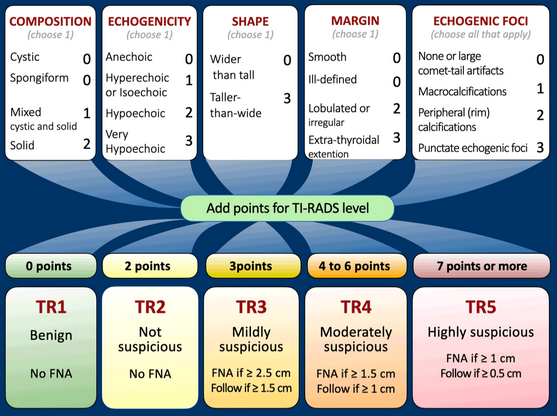
\includegraphics[width=1\linewidth]{images/tiradsACR.png}
        \caption{TIRADS Score}
        \label{fig:tiradsACR}
    \end{figure}

    \noindent
    Based on the TI-RADS score, radiologists determine the need for further diagnostic procedures, such as fine-needle aspiration biopsy (FNAB), to confirm or rule out thyroid cancer. This systematic approach ensures a more accurate and efficient evaluation of thyroid nodules, aiding in timely and appropriate clinical decision-making. \par \noindent
    \noindent The dataset contains multiple samples of different patients’ thyroid glands from different views, which are classified as per the TIRADS score.

    \begin{figure}[ht]
    \centering
    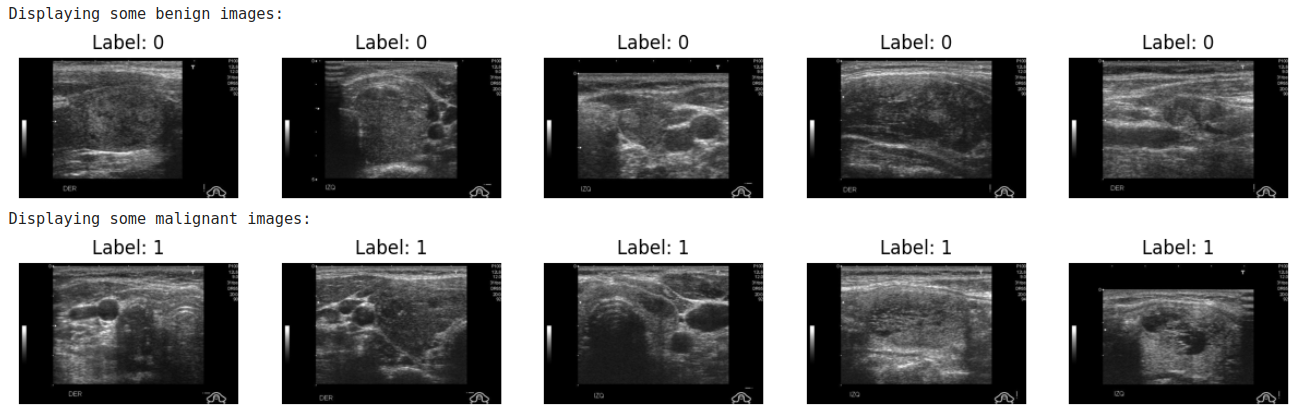
\includegraphics[width=\textwidth]{images/dataset.png}
    \caption{Sample of Ultrasound images from Dataset (0-Benign,1-Malignant).}
    \label{fig:thyroid_nodules}
\end{figure}
    \subsection{Data Preparation}
    \noindent
    All images in the dataset have a resolution of 560x360 pixels and are stored in a 24-bit RGB format (3 dimensions). Before being used as input for the Convolutional Neural Network (CNN), the images undergo preprocessing. This includes converting the images to an 8-bit unsigned integer (uint8) format and transforming them into grayscale, reducing the image to a single dimension. This preprocessing step ensures compatibility with the CNN model and optimises computational efficiency.
    \par \noindent During dataset preparation, the images are categorised into two classes: Benign and Malignant, based on their TI-RADS scores. Specifically, nodules with TR1 and TR2 scores are classified as Benign, as they indicate no or low suspicion of malignancy. On the other hand, nodules with TR3, TR4, and TR5 scores are categorised as Malignant, as TR3 represents mild suspicion, while TR4 and TR5 indicate moderate to high suspicion of malignancy. This classification ensures a clear distinction between benign and potentially cancerous nodules for training the model.
    \par \noindent The dataset is divided into training and testing subsets using the train-test split method. In the current approach, a test size of 0.2 is used, meaning 20\% of the dataset is allocated for testing, while the remaining 80\% is utilised for training the model. This split ensures a balanced distribution of data for evaluating model performance and generalisation.

    \section{CNN Model}
    \noindent
    The Convolutional Neural Network (CNN) is a specialised architecture within the domain of Deep Learning, specifically designed to interpret and analyse visual data. Unlike traditional Artificial Neural Networks (ANNs), which struggle to process raw image data directly, CNNs leverage the convolution operation as a fundamental image processing layer. This operation enables the network to automatically extract spatial features, such as edges, textures, and patterns, from images, making CNNs highly effective for tasks like image classification. By hierarchically learning these features, CNNs can understand complex visual information, outperforming ANNs in tasks involving image data. As a result, CNNs have become the preferred choice for image classification and other computer vision applications. \par \noindent
    The pooling layer plays a crucial role in downsampling the feature maps generated by the convolutional layer, reducing their spatial dimensions while retaining essential information. Following this, the dense layer (fully connected layer), like layers in an Artificial Neural Network (ANN), processes the feature maps. Before being fed into the dense layer, the feature maps are flattened into a 1-dimensional array. The dense layer then interprets these features to produce the final output, typically in the form of class probabilities, enabling the model to make predictions. Figure \ref{fig:CNN} shows the basic flow of the image data across the CNN model. Here, only three layers have been shown, but actual CNN models may contain multiple convolutional and maxpool layer and their multiple configurations. 

    \begin{figure}
        \centering
        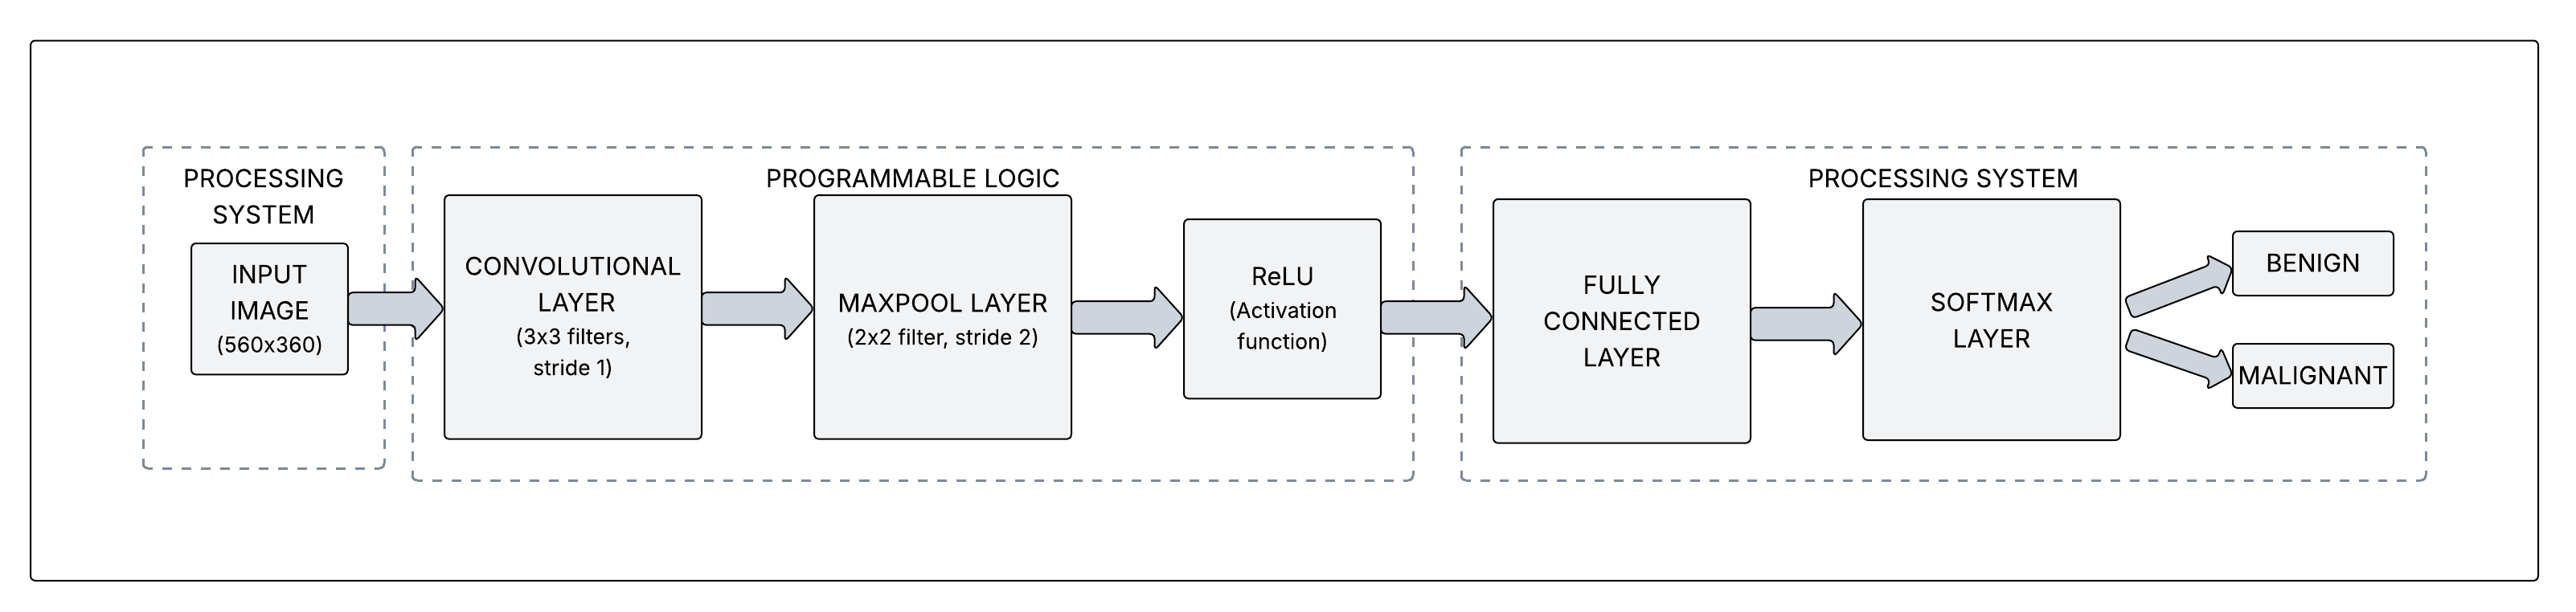
\includegraphics[width=1\linewidth]{images/block diagram overall.png}
        \caption{Overall block diagram}
        \label{fig:overall block diagram}
    \end{figure}

    \section{Hardware Software Partitioning}
    \noindent
    The PYNQ Z2 board belong to the ZYNQ-7000 SoC family of FPGA by Xilinx (now AMD), which integrates the software programmability of an ARM-based dual-core processor with the hardware programmability of an FPGA. The ARM processor is commonly referred to as the PS, whereas the FPGA fabric, where all the LUTs, BRAMs \& DSPs are present, is referred to as PL. There are several interfaces available for the PS and PL to communicate with one another. The PS is programmed in a high-level language like C/C++, and the PL is programmed using HDL languages or Xilinx IP cores, hence PS is known as Software, and the PL is known as Hardware. While designing an accelerated application the application should be partitioned to have maximum benefit from the PS as well as the PL, the PL is very good at performing compute-intensive tasks because of its parallelism capabilities however it performs weakly in tasks which are memory intensive, but the PS can handle the memory intensive tasks very well as compared to the PL. \par \noindent
    The CNN model involves mainly three distinct layers the convolutional layer, the pooling layer and the dense/fully connected layer keeping in mind the points mentioned above the CNN model is partitioned to achieve a better acceleration scheme all three layers are highly compute-intensive but the convolutional layer and pooling layer are very less memory intensive, the convolutional layer involves only a few amounts of weights biases which need to be stored on the PL and the pooling layer has no weights and bias associated to it thus this fact makes them suitable for the implementation of these layers on PL while the fully connected layer consists of a large number of weights and biases associated to it thus making it less ideal for PL implementation and more suitable for PS implementation. Thus, the convolutional layer and pooling layer are partitioned on the PL, while the fully connected layer is partitioned on the PS.
    \begin{figure}
        \centering
        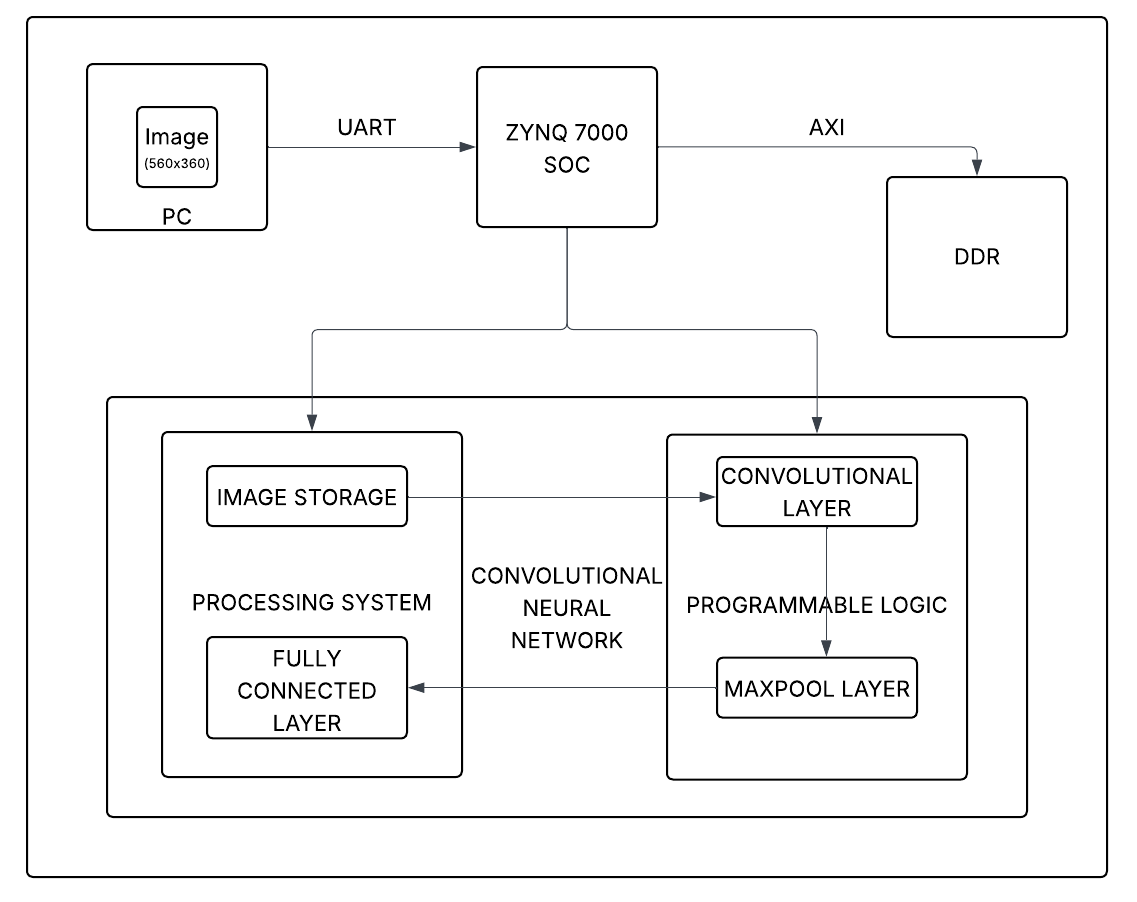
\includegraphics[width=0.8\linewidth]{images/diag_final.png}
        \caption{Hardware software partitioning}
        \label{fig:Hardware Software partitioning}
    \end{figure}
    
    \section{FPGA for Hardware Acceleration}
    \noindent
    The CPU manages diverse tasks efficiently, though it sequentially processes instructions, it has limited capacity for parallel processing and low performance in compute-intensive scenarios. The GPU, or Graphics Processing Unit, is built with many cores optimised for parallel processing. Still, this capability often comes at the cost of higher power consumption, a notable trade-off in its design. The FPGA is composed of a network of CLBs linked through programmable interconnects, thus increasing flexibility through reconfigurability, and could employ parallelism for accelerating operations.

    
    
    \section{Graphical User Interface}
    \noindent
    The FPGA is a very low-level device, it has a lot of peripherals available to it, but to use those peripherals, all of those need to be configured, having configured those interfaces, it is necessary that at the user level, the peripherals must be accessible easily to be able to communicate with the FPGA thus, a GUI needs to be developed. The GUI helps create a proper interface between peripherals and the user.

    \section{Workflow and Timeline}
    
    \subsection{Workflow}
    \begin{figure}[H]
        \centering
        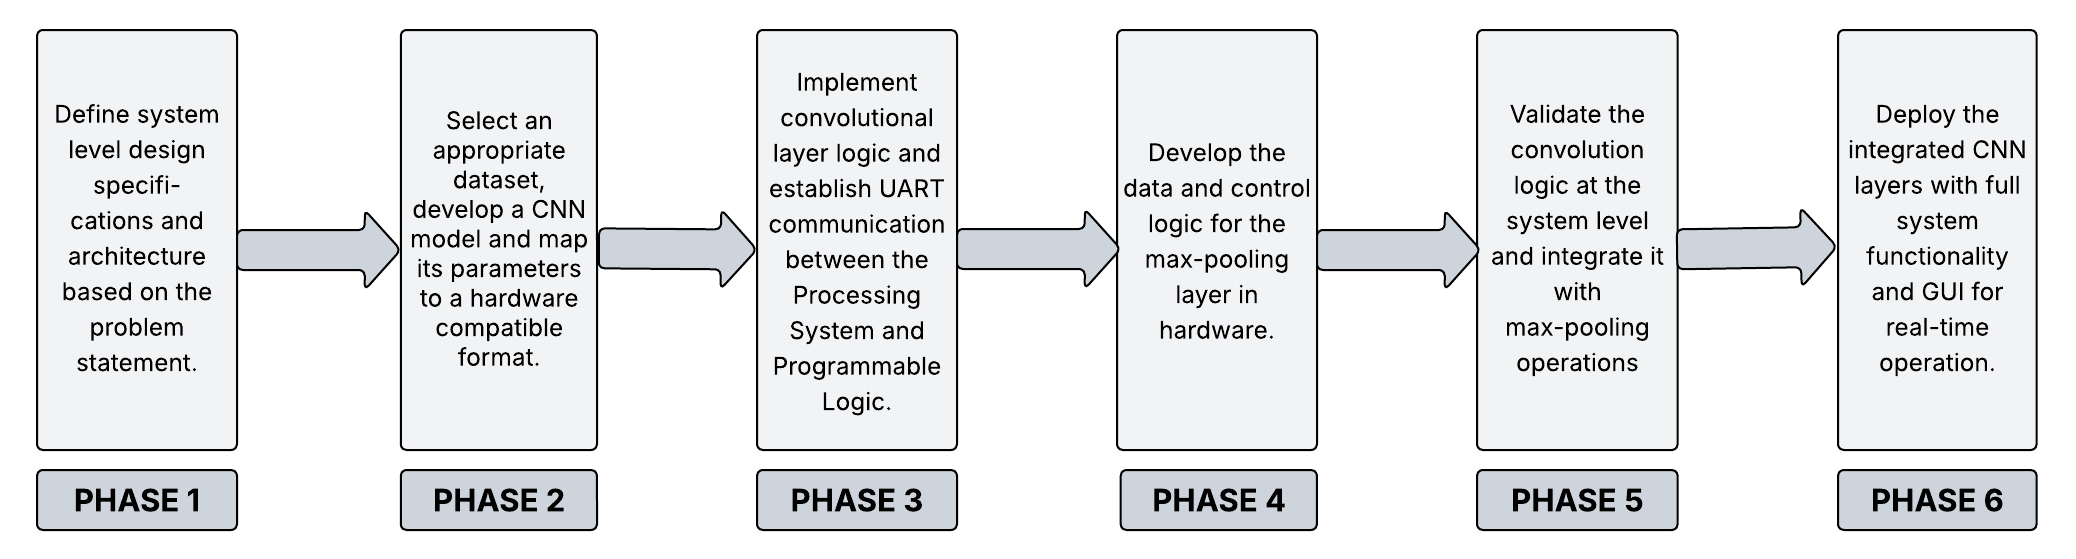
\includegraphics[width=1.1\linewidth]{images/workflow.png}
        \caption{Workflow}
        \label{fig:workflow}
    \end{figure}

    \subsection{Timeline}
    \begin{figure}[H]
        \centering
        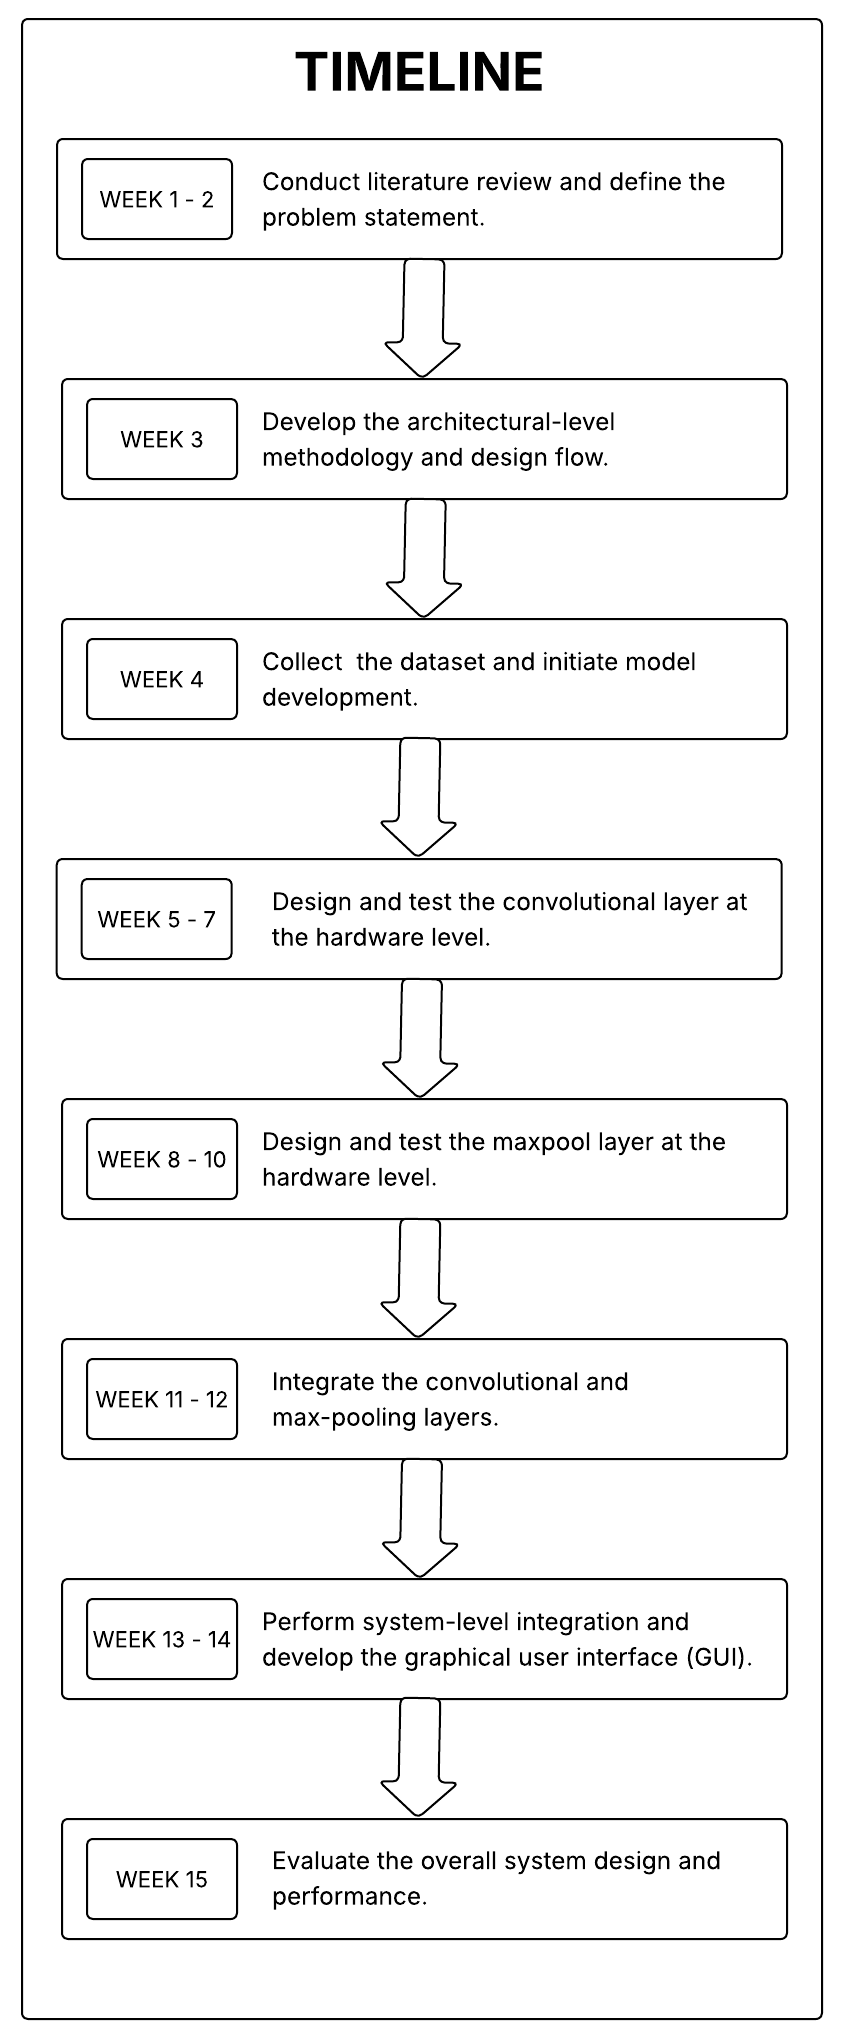
\includegraphics[width=0.57\textwidth]{images/timeline_final.png}
        \caption{Project Timeline}
        \label{fig:timeline}
    \end{figure}
    \newpage
    
    
    
    



    
    


 \newpage
\chapter{Design} 

\section{Convolutional Neural Network}
    \subsection{CNN Model Architecture}
    \noindent
    One of the most popularly used CNN model architectures is the VGG19 (Visual Geometry Group) architecture. It consists of 19 weight layers comprising 16 convolutional layers and 3 fully connected layers. The key components of the VGG19 architecture are:
    \begin{enumerate}
        \item Convolutional Layers: 3x3 filters with a stride of 1 and padding of 1.
        \item Activation function: ReLU (Rectified Linear Unit) applied after each convolutional layer.
        \item Pooling layers: Maxpooling layers with a 2x2 filter and a stride of 2.
        \item Fully connected layers: Three fully connected layers at the end of the network, at the end of classification.
        \item Softmax Layer: Final layer for classification with probabilities.
    \end{enumerate}
    The architecture of the CNN model consists of multiple key layers, including convolutional layers, pooling layers, and dense (fully connected) layers. The convolutional layer is responsible for feature extraction, utilising the Rectified Linear Unit (ReLU) activation function to introduce non-linearity and enhance the learning of complex patterns. To reduce the spatial dimensions and computational complexity while retaining the most essential features, max pooling is applied. This operation selects the maximum value from a defined window, preserving crucial information. Following the convolutional and pooling layers, a flattening layer is used to convert the multi-dimensional feature maps into a one-dimensional vector, which is then passed to the dense layer. The dense layer is fully connected, meaning each neuron in one layer is linked to every neuron in the next layer. This layer utilises the softmax activation function for classification, enabling the model to output probability distributions corresponding to benign or malignant categories. \par \noindent
    The CNN model is implemented using Python with the TensorFlow machine learning framework, which provides a comprehensive set of tools for designing, training, and optimising deep learning models. TensorFlow’s flexibility and efficiency allow for the seamless deployment of CNN-based solutions for real-time decision-making in thyroid nodule classification.

    \begin{figure}[ht]
        \centering
        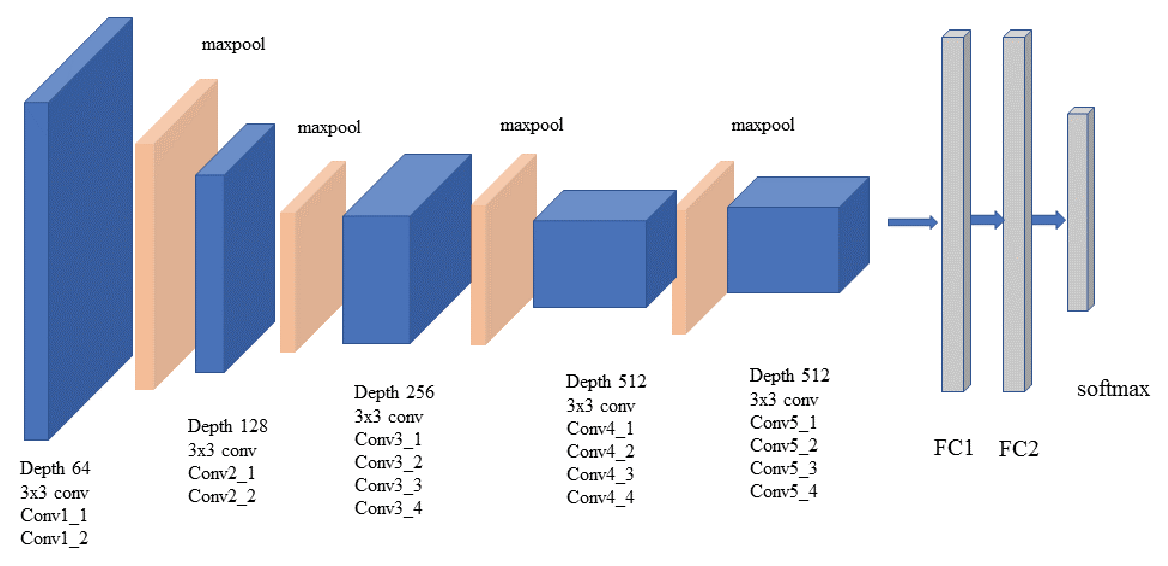
\includegraphics[width=0.75\linewidth]{images/vgg19.png}
        \caption{The VGG19 model architecture}
        \label{fig:vgg19}
    \end{figure}

    \subsection{CNN FPGA Deployment}
    \noindent
    As the number of layers increases, the model requires more compute resources, and the FPGA used, i.e. PYNQ Z2, has a limited number of resources. Thus, it may not be possible to deploy a large model, along with the fact that the design, development and testing of the implementation at the FPGA level is a very time-consuming task. Hence, for the sake of simplicity and considering the above points, this project uses a simple 3-layer Convolutional Neural Network Architecture consisting of a Convolutional layer, Maxpool layer and a dense layer for FPGA Deployment, and at each stage \textit{relu} is used as an activation function. The model summary of the model being considered for deployment is shown in figure \ref{fig:model_summary}. Figure  \ref{fig:CNNpartition} briefly illustrates the partitioning of the CNN model acceleration scheme for the model under consideration. Along with other partitioned tasks being employed in the partitioning scheme.

    \begin{figure}
        \centering
        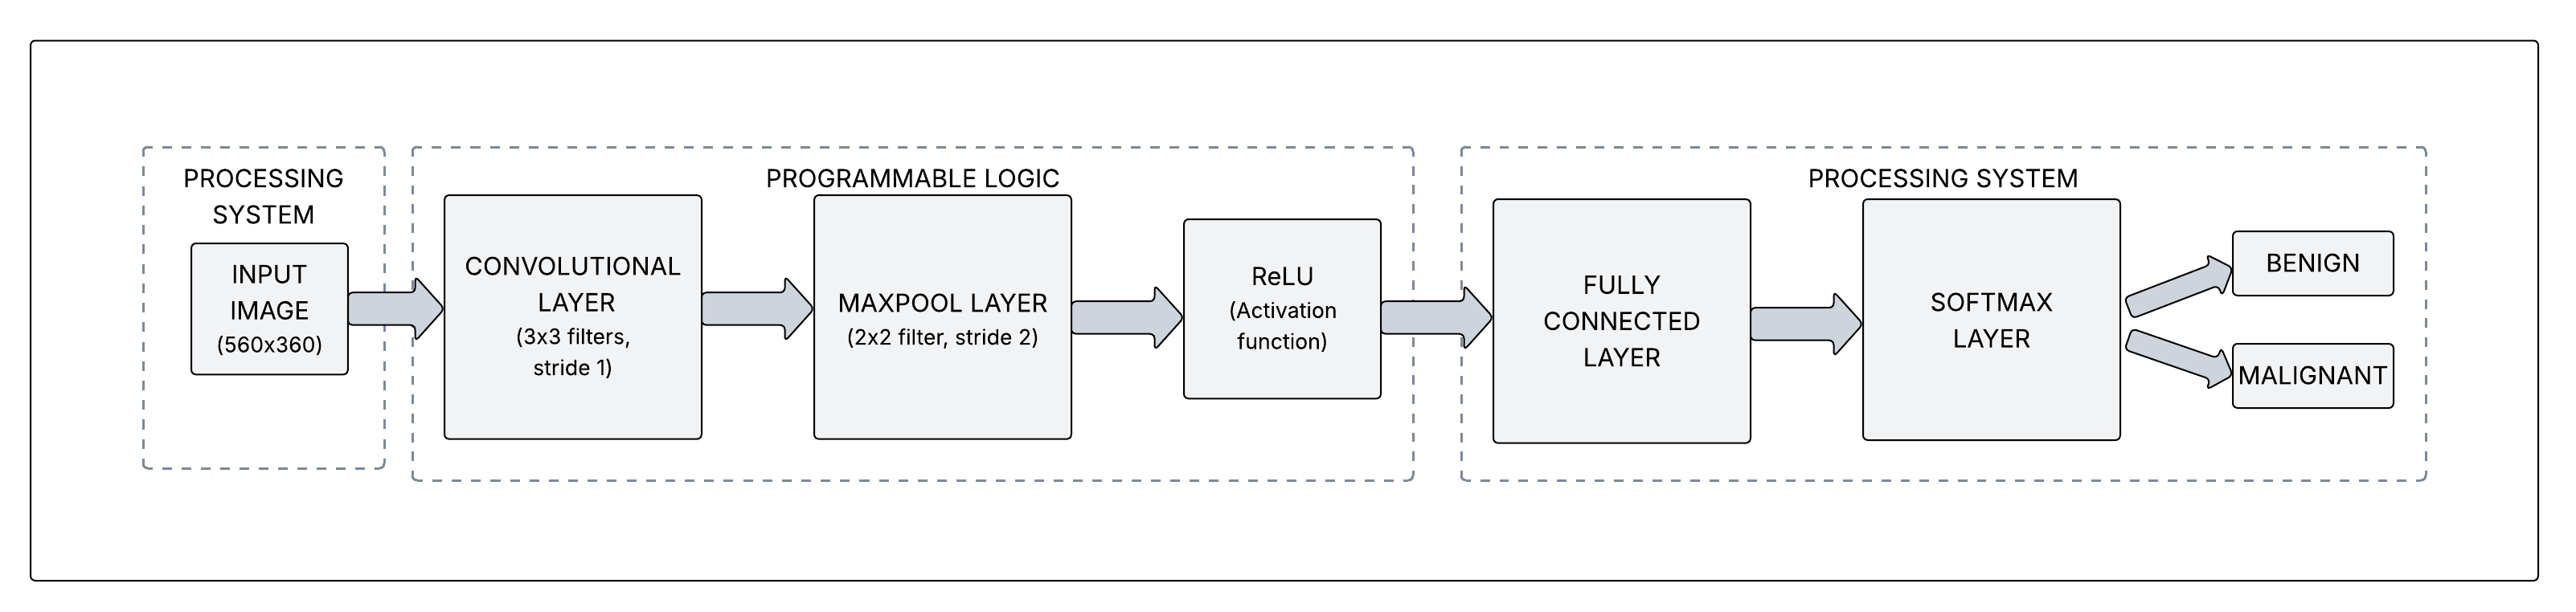
\includegraphics[width=1\linewidth]{images/newCNNdiag.png}
        \caption{CNN Model and Partitioning scheme}
        \label{fig:CNNpartition}
    \end{figure}
    
    \begin{figure}[H]
    \centering
    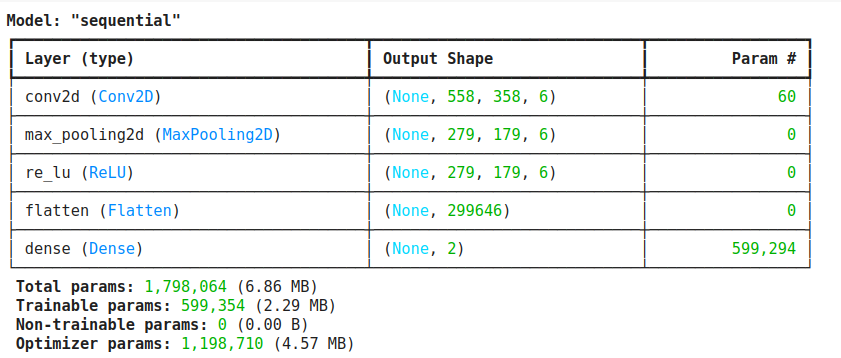
\includegraphics[width=\textwidth]{images/model_summary.png}
    \caption{Model Summary Table}
    \label{fig:model_summary}
    \end{figure}

    \section{Processing System}
    \noindent
    The processing system (PS) refers to the processor on the PYNQ Z2, which is an ARM Cortex A9 dual-core processor. As mentioned earlier, this is used for implementing the fully connected layer. The PS, apart from computing the result from the fully connected layer, is also responsible for receiving the input image for classification through the UART interface and then transferring it to the PL using the DMA. The top module collects data from the DMA, which transfers the data through the AXI MM2S interface, which is shown in Figure \ref{fig:overall_block}.

    \begin{figure}[H]
    \centering
    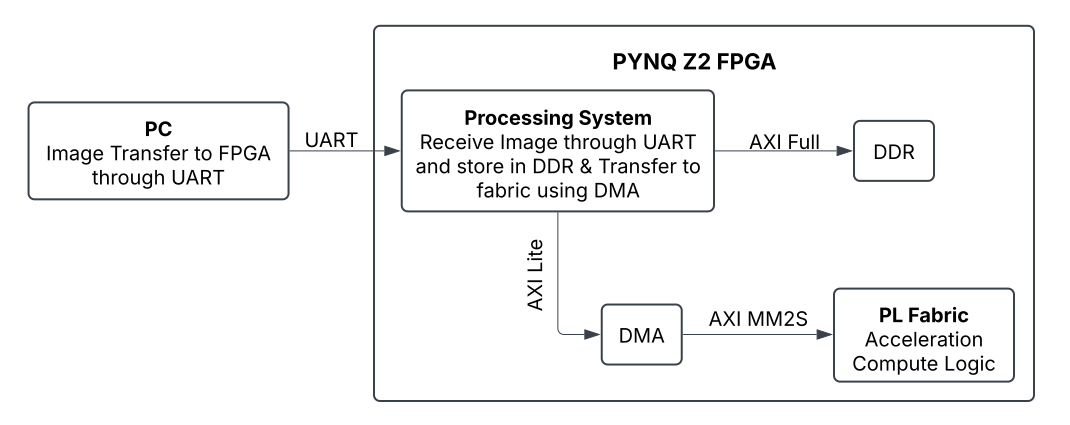
\includegraphics[width=\textwidth]{images/OverallBlockDiagram.png}
    \caption{Overall high-level view of FPGA acceleration scheme}
    \label{fig:overall_block}
    \end{figure}

    \section{AXI Protocol}
    \noindent
    The AXI protocol is widely used across the system design of the entire project. The AXI protocol comes in three variants: 
    \begin{enumerate}
    % \setlength{\itemsep}{0.5pt}
    % \setlength{\parskip}{0.5pt}
    % \setlength{\topsep}{0.5pt}
    \item AXI Full
    \item AXI Lite
    \item AXI Stream
    \end{enumerate}
    \noindent
    Out of which the first two are memory-mapped interfaces, while AXI Stream is not, making it a simpler one among the three to implement and reducing memory overhead, thus the acceleration logic deployed on the fabric uses an AXI Stream protocol. The DDR, being a memory-mapped peripheral, communicates with the PS using the AXI Full protocol, whereas DMA, which is also a memory-mapped interface, communicates with the PS through the AXI Lite interface. Now that our PL logic is based on the AXIS protocol, the DMA, which consists of bridging logic, communicates with PL through AXI MM2S (memory-mapped to stream) interface. Figure \ref{fig:AXI_Stream_block} shows a simple interface between two AXI Stream peripherals, with ready, valid and data signals, apart from the clock and reset, other signals are optional and hence not shown. Figure \ref{fig:axi_stream_waveform} shows AXIS protocol waveforms, only the ready, valid and data signals are taken in our implementation, as the rest of the signals are optional.

    \begin{figure}
        \centering
        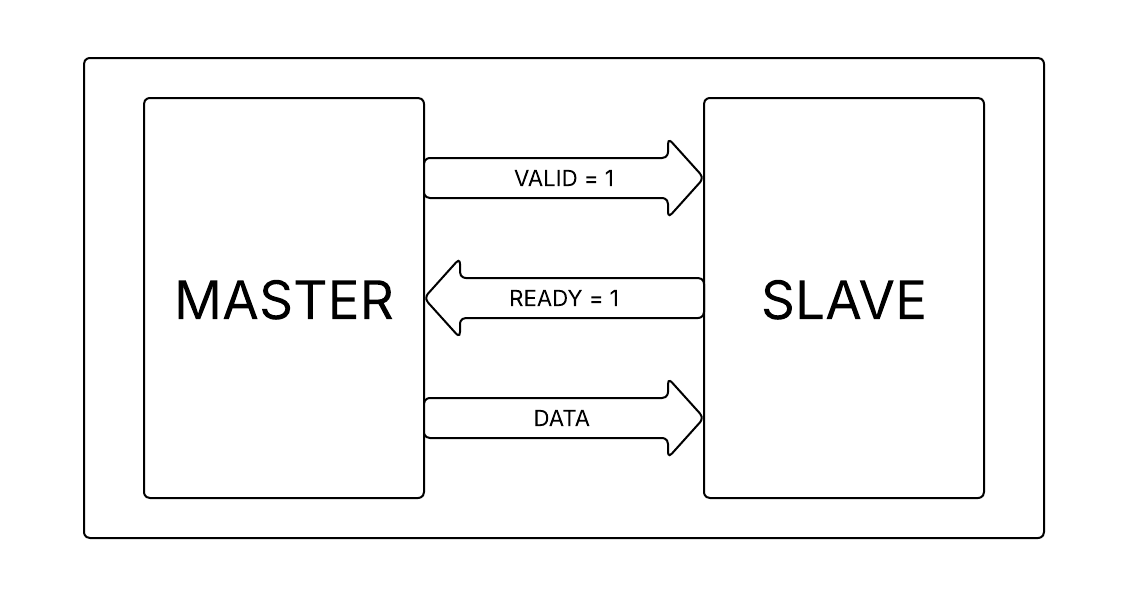
\includegraphics[width=0.75\textwidth]{images/axi_image.png}
        \caption{AXI Stream block interface}
        \label{fig:AXI_Stream_block}
    \end{figure}

    
    \begin{figure}[H]
    \centering
    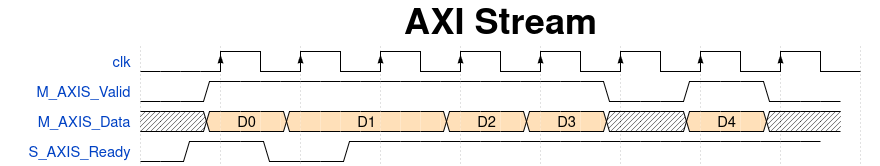
\includegraphics[width=\textwidth]{images/AXI_StreamWaveDrom.png}
    \caption{AXI Stream Protocol Waveform}
    \label{fig:axi_stream_waveform}
    \end{figure}

    \section{PL Fabric}
    \subsection{Data Representation}
    \noindent
    The CNN model when designed on PC uses float32 format to store the weights and biases which are associated with the convolutional and fully connected layer but using float representation on FPGA would be very expensive considering the amount of available resources for logic implementation so a fixed point scheme is adopted instead where MSB represents the sign bit and following three bits represent integer part and remaining bits represent the fraction bits. The integer bits are 3 bits wide because the weights and biases are not larger than the possible range of representation. Further, after certain computations such as multiplication or addition, the integer width is adjusted to accommodate the result adequately without loss of significant bits. Figure \ref{fig:fixed_point} shows the fixed point representation, width and bit position.

    \begin{figure}[ht]
    \centering
    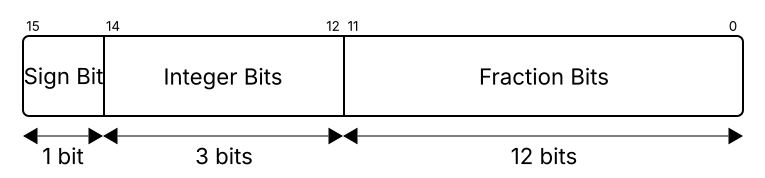
\includegraphics[width=\linewidth]{images/Data_16Bit_Representation.png}
    \caption{Data Representation for Weight \& Biases}
    \label{fig:fixed_point}
    \end{figure}

    \subsection{Convolution Layer Architecture} \label{sec:conv_architecture}
    \noindent

    \begin{figure}[H]
        \centering
        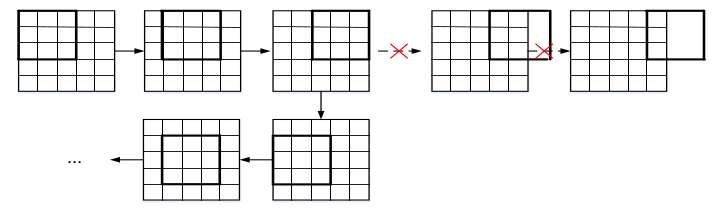
\includegraphics[width=\textwidth]{images/conv_window.png}
        \caption{Convolution operation window}
        \label{fig:conv_window}
    \end{figure}

    \noindent Figure \ref{fig:conv_window} shows how the filter moves across the image in a convolution operation, and is modelled to operate the same way at the hardware level.
    The convolutional layer uses 4 line buffers to store the data required for the convolution operation as shown in figure \ref{fig:line_buffer_architecture}, one line buffer stores data from one row of the image, since the kernel is a 3x3 kernel at least 3 line buffers are required for the operation, while 3 line buffers are being read one line buffer is storing data from the PS. The 4-line buffer structure takes one pixel of image data at every clock edge. The three-line buffers, which are being read, give data of 3x3, i.e. 9-pixel values, 8 bits wide, which is 72 bits wide. The modelling of the convolution operation is discussed in more detail in the subsequent section, as the data and control logic, as a whole, the convolution operation is wrapped in a top module comprising both data and control logic.
    
    

    \begin{figure}[H]
    \centering
    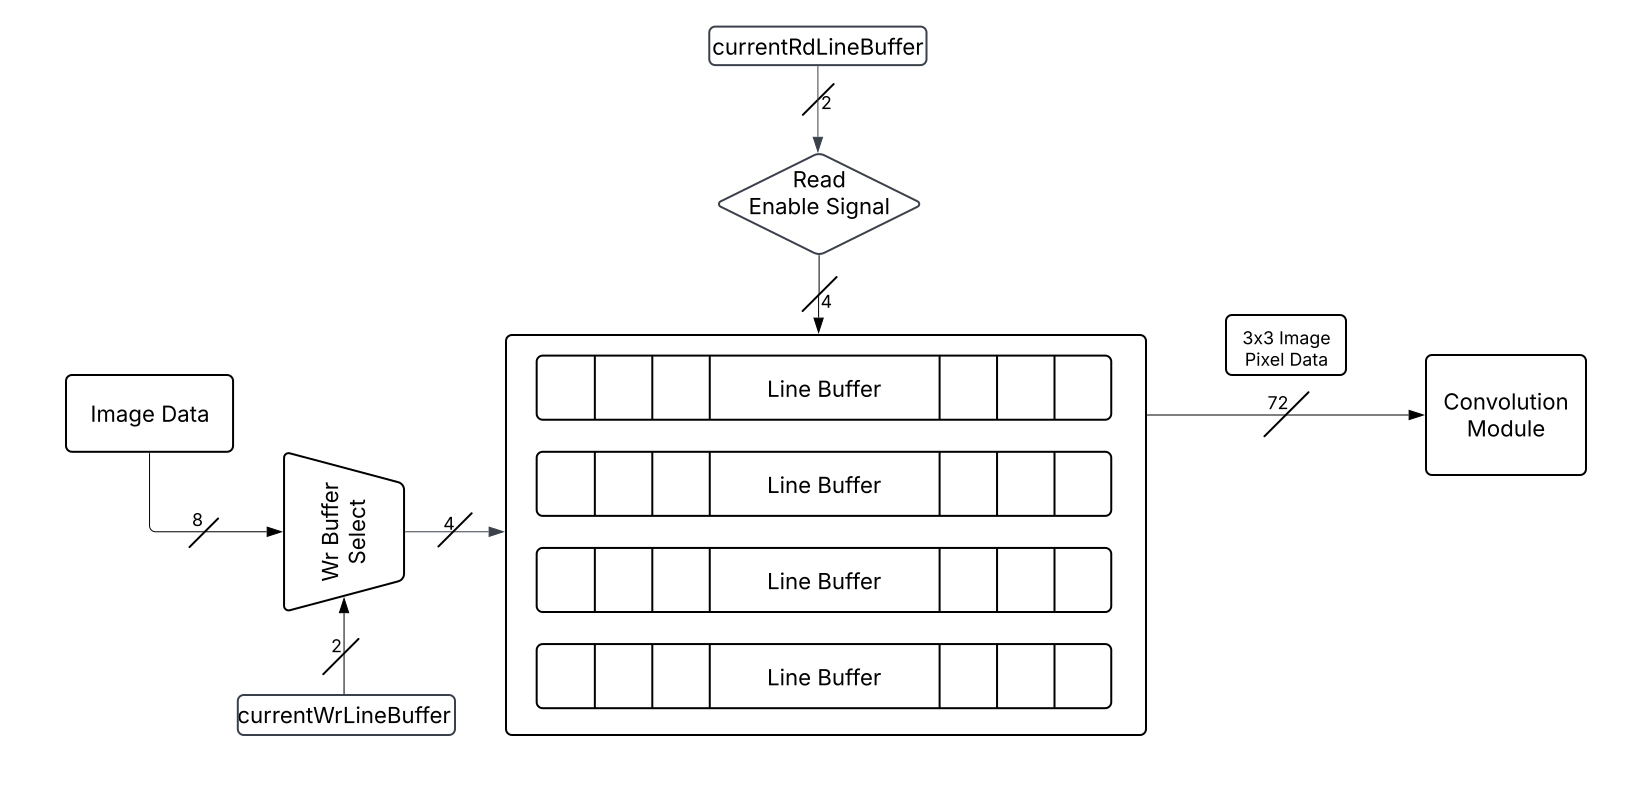
\includegraphics[width=\linewidth]{images/CONV_Architecture.png} 
    \caption{Convolution Layer line buffer architecture}
    \label{fig:line_buffer_architecture}
    \end{figure}

    \noindent
    \subsubsection{Data Logic}
    \noindent
    The convolution module upon receiving the data from line buffers computes the result for one set of 3x3 pixels in 4 stages which are shown in figure \ref{fig:pipeline_architecture}, in the first stage all the data is multiplied in a parallel fashion and stored in 9 registers(0-9) shown in figure \ref{fig:pipeline_architecture} in the second stage, these are added 3 at a time and their results are stored in 3 registers(Sum1, Sum2 \& Sum3) shown in the figure \ref{fig:pipeline_architecture} this addition occurs as soon as the multiplication results are available that is achieved because this stage is modelled in a combinational manner to reduce one clock latency, the next stage sums the data in those 3 registers to generate the convolution result, the fourth stage performs \textit{relu} operation which is an activation function and adds the bias to the result of convolution. The stagewise completion of the convolution operation is indicated by the \textit{valid} signal, which propagates through stages, the \textit{valid} signal going high at the final stage means the convolution operation result is available. The result of the convolution is 24 bits wide, MSB as the sign bit followed by 11 bits of integer part and remaining bits to represent fraction part, is shown in figure \ref{fig:conv_result}.

    \noindent The equation given below shows the \textit{relu} operation.

    \[
    f(x) =
    \begin{cases} 
    x & \text{;  } x > 0 \\
    0 & \text{;  } x \leq 0
    \end{cases}
    \]

    \begin{figure}[H]
    \centering
    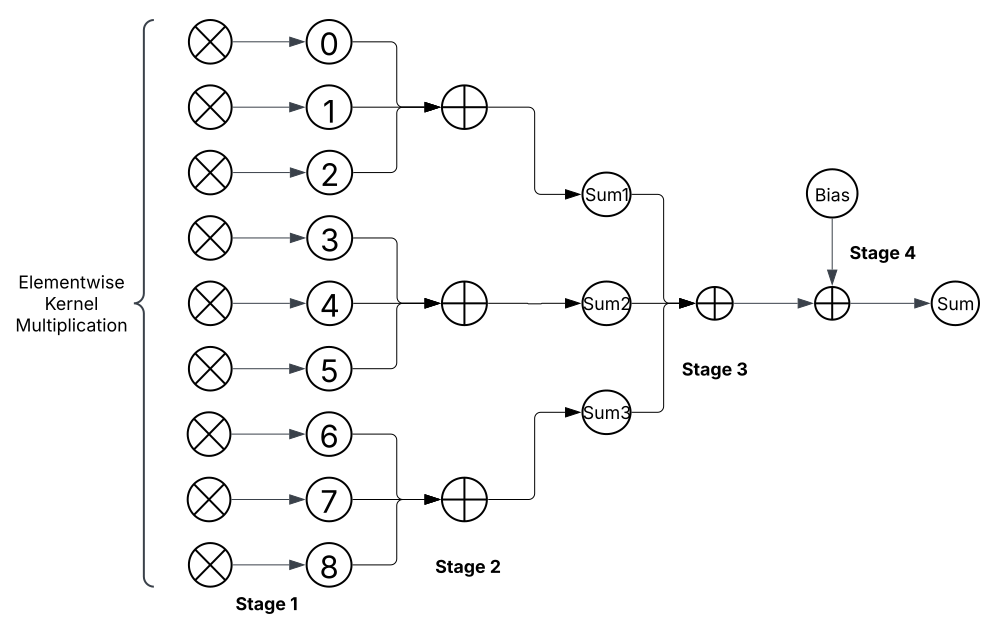
\includegraphics[width=\linewidth]{images/MAC_Unit.png} 
    \caption{The Convolution operation stagewise implementation scheme}
    \label{fig:pipeline_architecture}
    \end{figure}

    \begin{figure}[H]
        \centering
        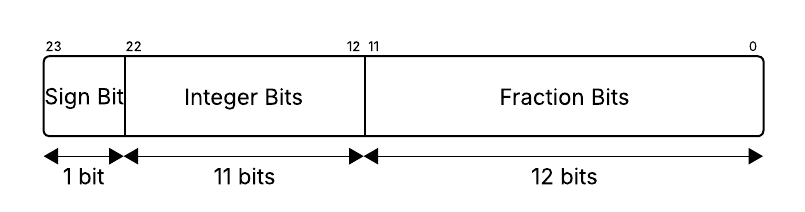
\includegraphics[width=\textwidth]{images/conv_result.png}
        \caption{Convolution result width format}
        \label{fig:conv_result}
    \end{figure}

    \subsubsection{Control Logic}
    \noindent
    One point to note in convolution operation is inorder to compute convoluted result 3 rows of data i.e. 3 line buffers must be ready with the data, figure \ref{fig:threeLineBuffcontrol} shows the state diagram for the same, the totalPixelCounter counts whether three line buffers have been filled or not by monitoring the input valid signal \textit{i\_data\_valid} while data is not being read, totalPixelCounter as shown in figure does not update its count while read and write occur simultaneously since it means one pixel is being written and one is being read so total pixel count does not change, while no data is being read totalPixelCounter decrements. 

    \begin{figure}[H]
    \centering
    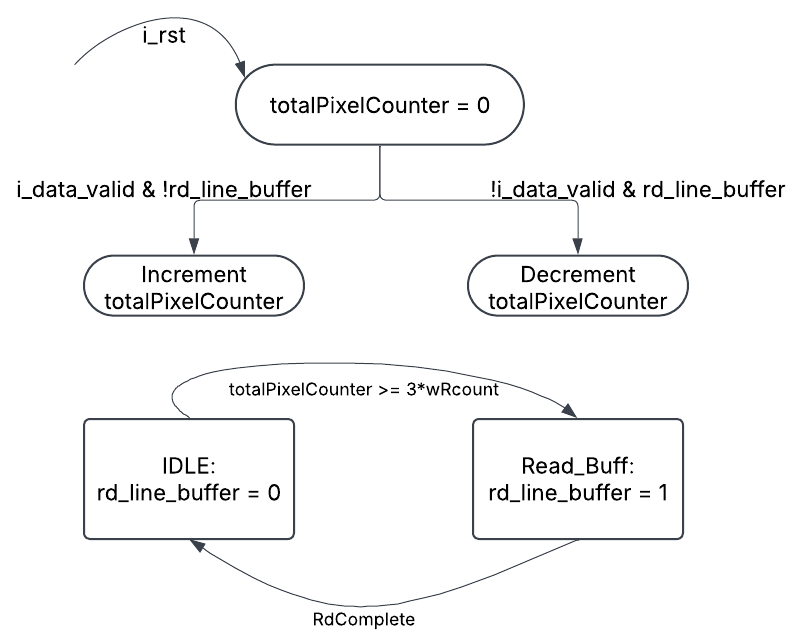
\includegraphics[width=0.75\linewidth]{images/readTotalCount.png}
    \caption{Control logic for read signal}
    \label{fig:threeLineBuffcontrol}
    \end{figure}

    \noindent
    The convolution operation involves shifting the kernel, which is handled by the control logic. The ‘currentWrlinebuffer’, ‘currentRdlinebuffer’ keep a track of which buffer to write new data and which buffers to read from. Figure \ref{fig:wrBufferControl} and \ref{fig:rDBufferControl} represent the counter and state diagram used to generate ‘currentWrlinebuffer’ and ‘currentRdlinebuffer’ signals.
    Here, wRcounter and Rdcounter have a similar task they go high whenever writing and reading, respectively, of a row is completed. These signals keep updating the ‘currentRdlinebuffer’ and ‘currentWrlinebuffer’, and the state of these two signals generates read and write \textit{valid} or, in simple words, enable signals. The reading operation reads three line buffers at a time in a cyclic fashion, while the write operation writes to one line buffer.

    \begin{figure}[H]
    \centering
    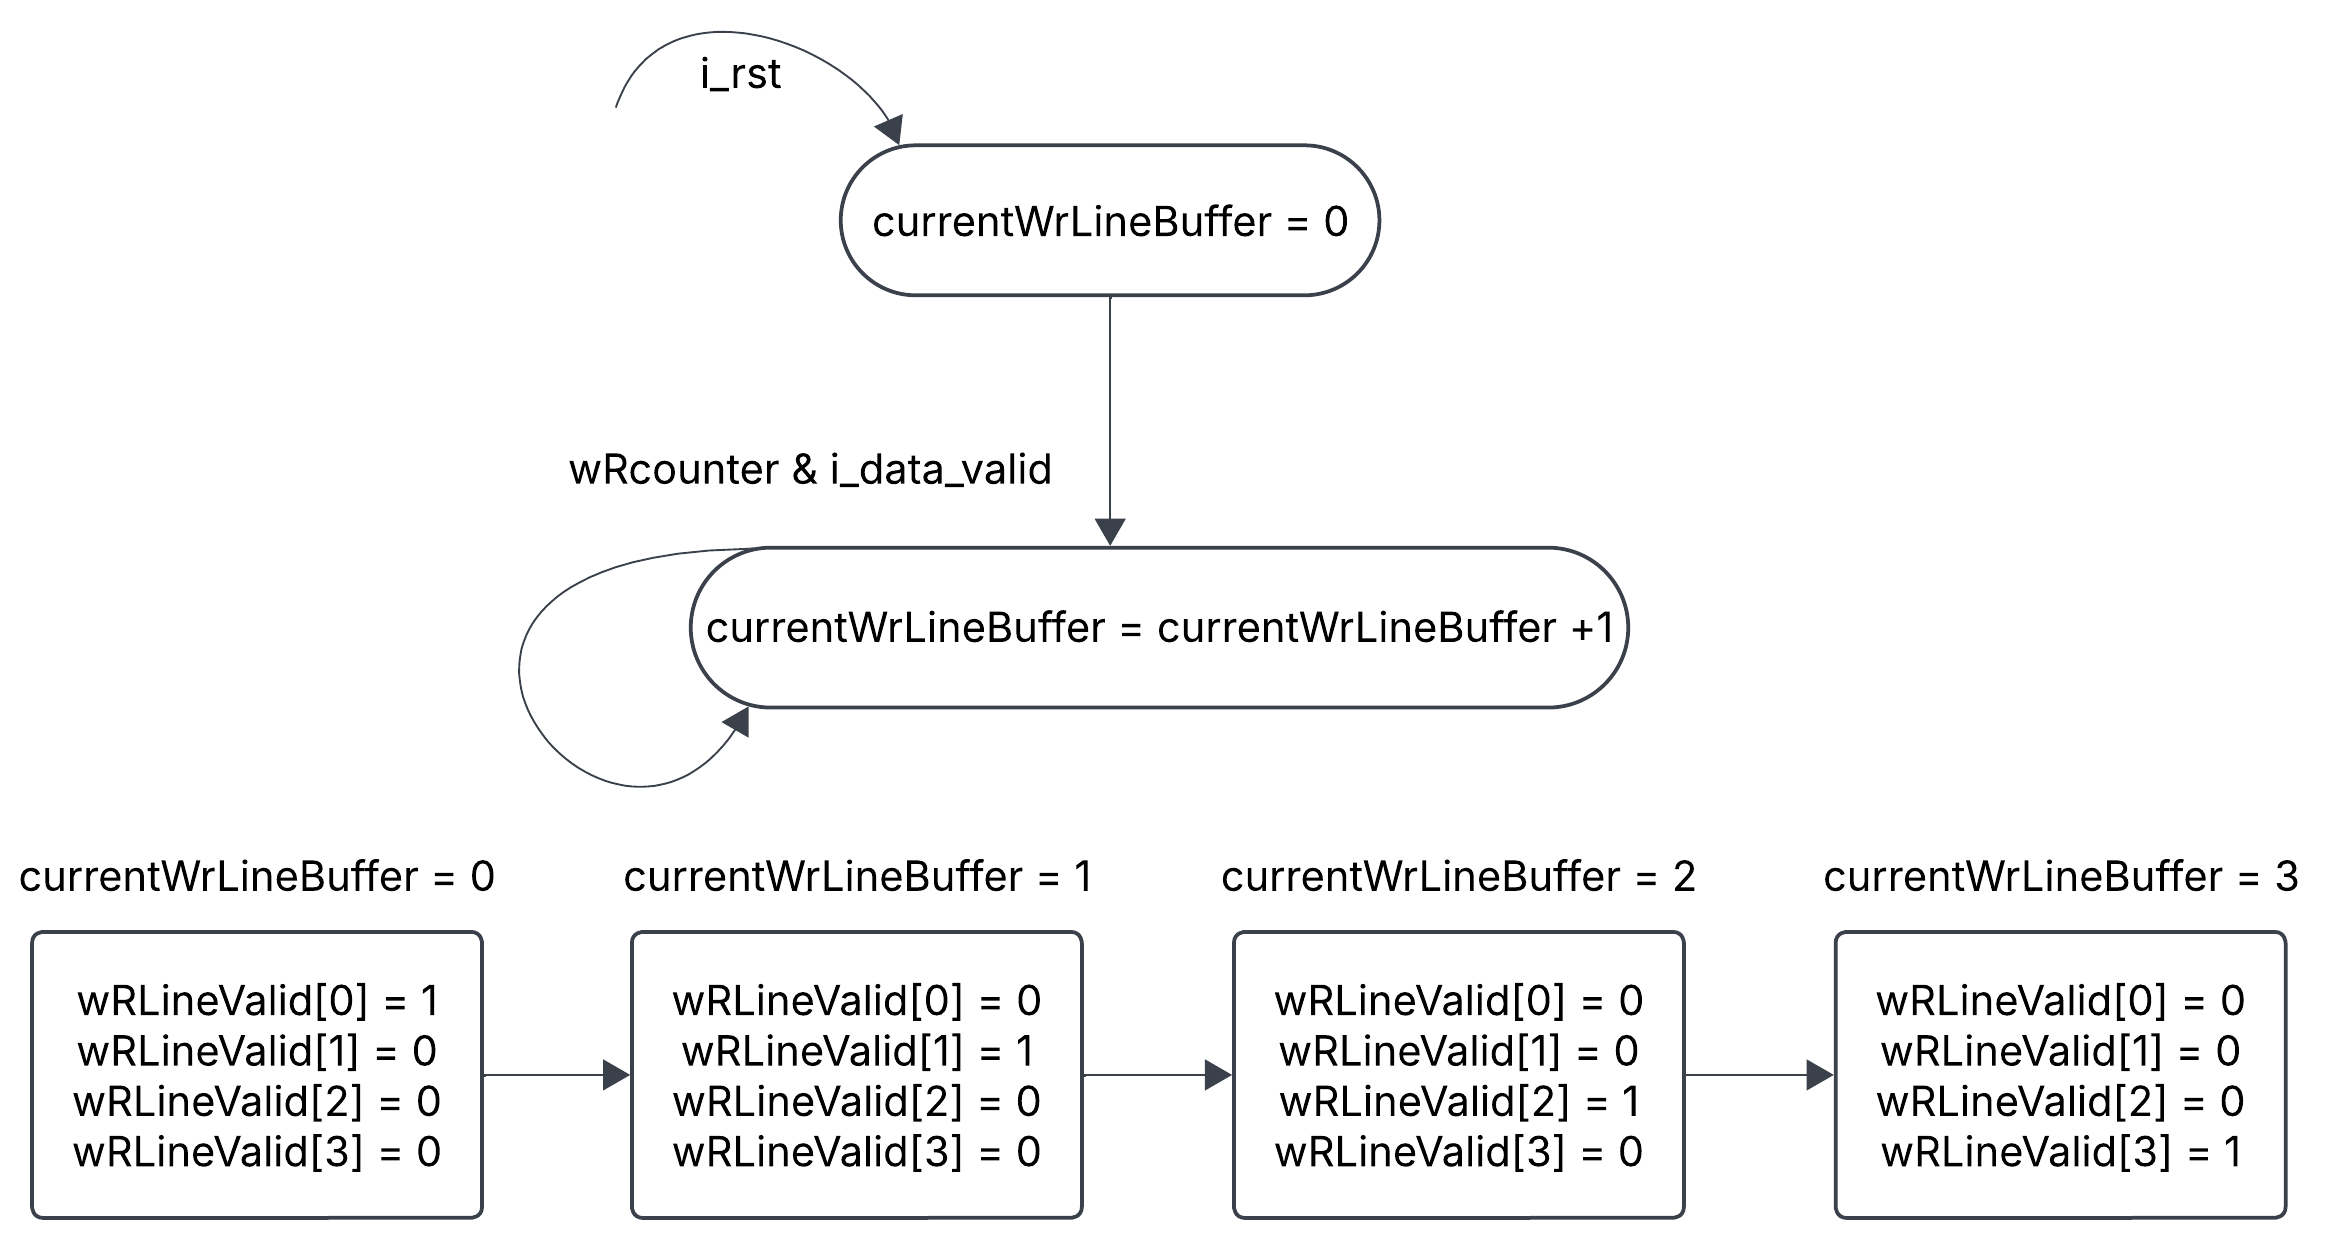
\includegraphics[width=0.75\linewidth]{images/convWrcontrol.png}
    \caption{Write Line Buffer counter and state diagram}
    \label{fig:wrBufferControl}
    \end{figure}

    \vspace{-1em}  % adjust this to control spacing

    \begin{figure}[H]
    \centering
    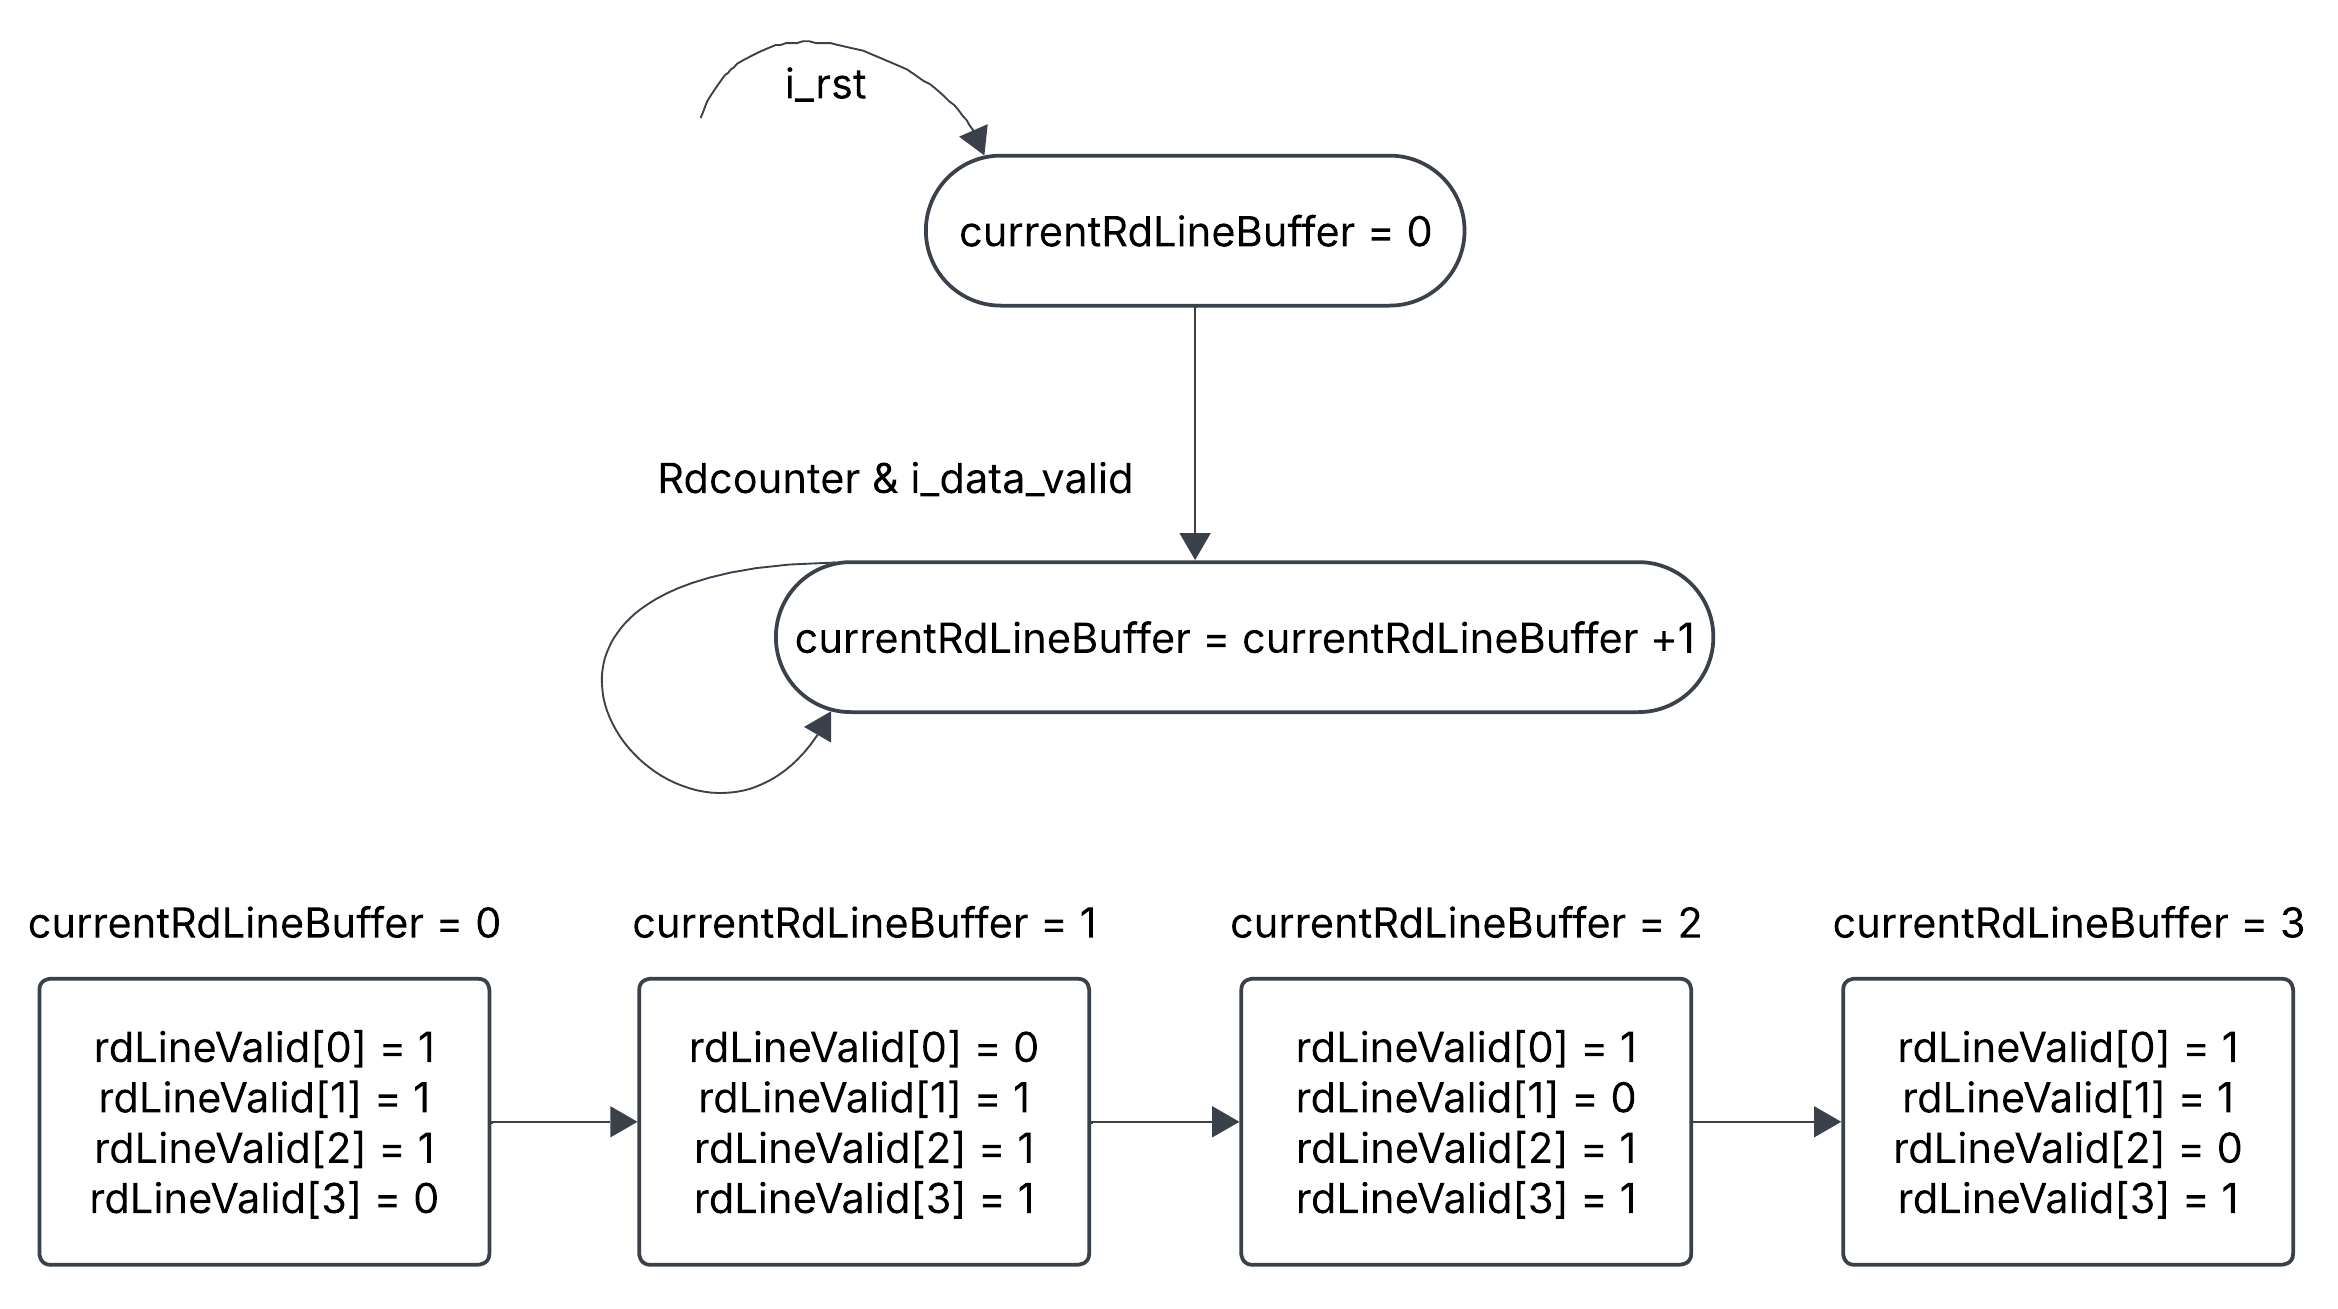
\includegraphics[width=0.75\linewidth]{images/convRdcontrol.png}
    \caption{Read Line Buffer counter and state diagram}
    \label{fig:rDBufferControl}
    \end{figure}


    \subsection{Maxpool Architecture}
    \noindent
    The figure \ref{fig:maxpool_operation} shows the maxpool operation, of how the kernel moves across the image, and is modelled in the same way at the hardware level. The maxpool and convolution logic are connected through the AXI  Stream. The output of the convolutional layer, which is input for the maxpool layer, is 24 bits wide, where the MSB bit represents the sign of the number and the integer bits are 11 bits wide, followed by 12 bits of fraction as shown in the figure \ref{fig:conv_result}. The integer part is increased from 3 to 10 bits to accommodate the product of image data and kernel as discussed in \ref{sec:conv_architecture}. 
    \par \noindent
    One of the critical parts while designing the maxpool control logic is taking into account the fact that maxpool processes the convolution data at a faster rate than it receives it from the convolution logic, which is because of the stride of 2. Thus, ensuring an appropriate set of pixels in synchronisation with the input convolved data became a challenging task.
    \par \noindent
    The maxpool layer uses 4 line buffers to store the data required for the convolution operation, as shown in the Figure \ref{fig:max_buff_arch} here, one line buffer stores convolution data row-wise.  The kernel in the maxpool layer is of 2x2, thus at a time, two line buffers are processed. Also, there is a stride of two, hence another two buffers store the data for the next processing. The ‘currentWrlinebuffer’ and ‘currentRdlinebuffer’ are the signals which control data being transferred to the maxpool data logic. Since the maxpool simply involves a comparison operation and no addition, multiplication, the result is of the same width as the convolution result.
    
     \begin{figure}[ht]
        \centering
        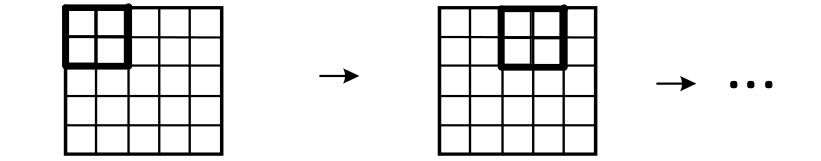
\includegraphics[width=0.75\linewidth]{images/maxpool.png}
        \caption{Maxpool Operation}
        \label{fig:maxpool_operation}
    \end{figure}
    
    \noindent The maxpool module, upon receiving the data from line buffers, computes the result for one 2x2 kernel in two stages as shown in Figure \ref{fig:stagewise_conv}. In the first stage, two pairs of data are compared with each other and the maximum of each respective pair is stored in an intermediate register, compIntm1 and compIntm2. The next stage computes the maximum of the maximum of two from the previous stage, which were stored in the intermediate registers.

    \begin{figure}[h!]
        \centering
        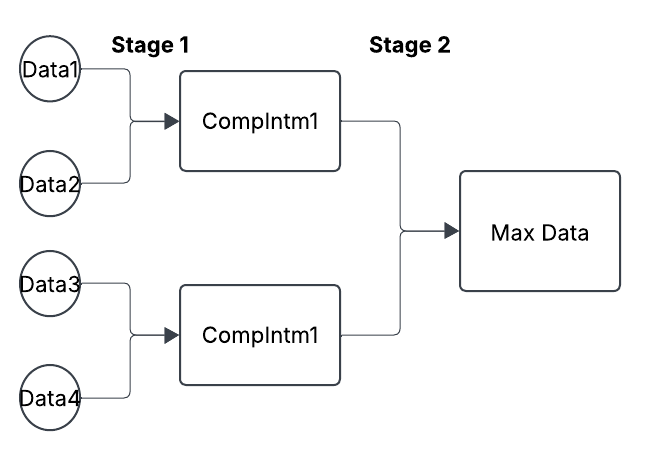
\includegraphics[width=0.75\linewidth]{images/stageWiseMax.png}
        \caption{Stagewise operation of Maxpool Layer}
        \label{fig:stagewise_conv}
    \end{figure}

    \begin{figure}[H]
        \centering
        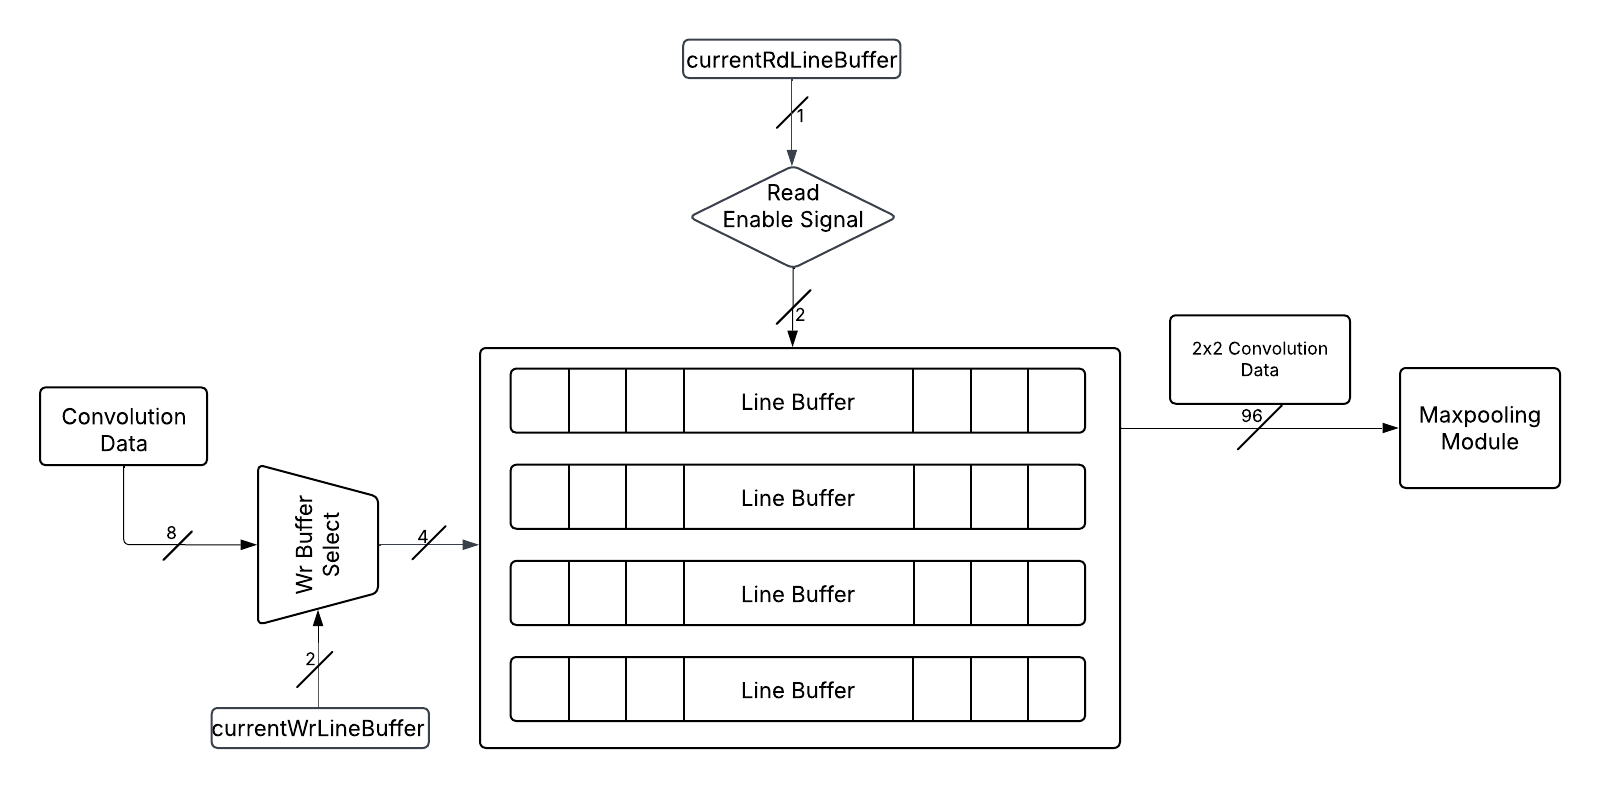
\includegraphics[width=\linewidth]{images/maxpool_architecture.png}
        \caption{Maxpool Buffer Architecture}
        \label{fig:max_buff_arch}
    \end{figure}
    
    \section{Overall Integration}
    \subsection{Convolution Maxpool Integration}
    \noindent
    Upon successful design and testing of the convolution and maxpool modules, they must be integrated for proper feature map generation. At the top level, both of the modules are designed around the AXI stream protocol interface, and thus are connected using the AXI stream interface. Since the fully connected layer is implemented at the PS level, the convolution and maxpool modules are combined to form a single AXI-based maxpooled data stream generating IP block. Figure \ref{fig:conv_max_integration} shows the interfacing between the convolution and maxpool module. It can be seen that all the signals, i.e. the ready, valid and data signals, are based on the AXI Stream protocol, the respective signals have been mapped to the appropriate ports according to the protocol.

    \begin{figure}[h]
        \centering
        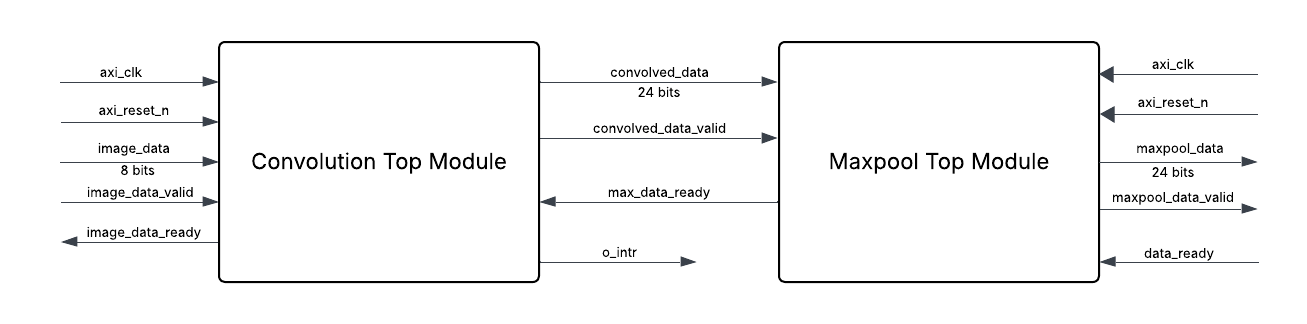
\includegraphics[width=1\linewidth]{images/conv_max_integration.png}
        \caption{Convolution Maxpool Integration}
        \label{fig:conv_max_integration}
    \end{figure}

    \subsection{Block Level Integration}
    \noindent
    After successful completion of design, integration and verification of the convolution and maxpool modules, the integrated design is packaged as a single IP using the Vivado IP Packager tool. This step is necessary to ensure that the convolution and maxpool as a whole design could be interfaced with the AXI DMA and the ZYNQ7 Processing System(PS). Creating the block design involves several steps, starting with configuring the IP repo to be able to use our packaged IP. In this stage majority of configurations are made, such as setting the Clock Frequency, PS UART baud rate, and enabling or disabling certain ports. The IP, which is created in this project, works on an AXI Stream protocol. DMA has an AXI\_LITE interface, using which it communicates with the PS. The interfacing between PS and the IP is enabled by the DMA, which connects to the IP through the AXI Stream MM2S and S2MM at the master port and slave port, respectively. As can be seen in the figure \ref{fig:convMaxBD}, an IP \textit{AXI Stream Data Width Converter} is used to interface master port of the IP and the slave port of the DMA, because the slave port of the master supports 32-bit data, and the output of the convolution is 24 bits wide.

    \begin{figure}[H]
        \centering
        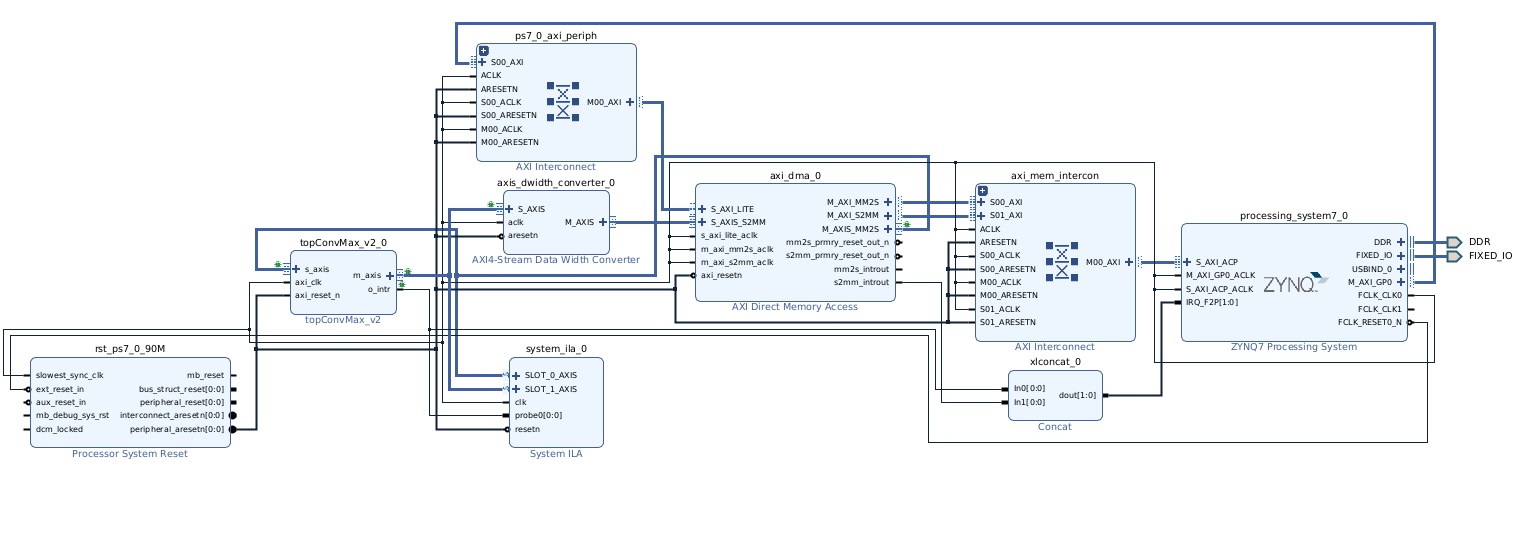
\includegraphics[width=1\linewidth]{images/convMaxBlockDesign.png}
        \caption{Convolution and Maxpool IP Block Design}
        \label{fig:convMaxBD}
    \end{figure}

    \noindent
    The following figure \ref{fig:addressMap} shows the address map for the memory-mapped interfaces. It can be verified from the address map that the appropriate ports are connected at the respective ports, and it also shows the addresses.

    \begin{figure}[H]
        \centering
        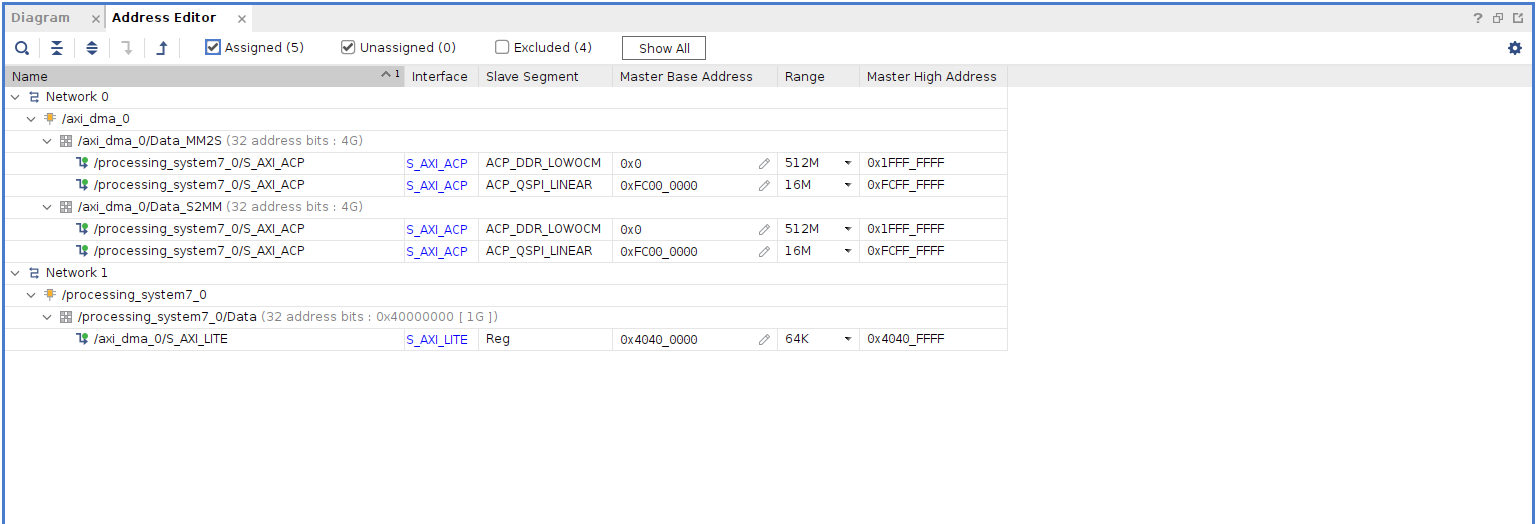
\includegraphics[width=1\linewidth]{images/addressMap.png}
        \caption{Address Map for memory-mapped interfaces}
        \label{fig:addressMap}
    \end{figure}
    \newpage
    
 \setlength{\parindent}{2em}

\chapter{Simulation \& Validation}
    \section{Simulation}
    \noindent
    Before packaging into IP and system-level integration, the RTL design is tested on some data to ensure the data and control units are working properly and give the desired result from the convolution operation. 

    \noindent The following kernel is chosen for simulation purposes, and the bias value is taken as:
    
    \begin{center}
    \begin{tabular}{|c|c|c|}
    \hline
    -0.03322114422917366 & -0.18549901247024536 & -0.25089457631111145 \\ \hline
    0.025202458724379539 & 0.15725375711917877 & 0.044544823467731476 \\ \hline
    0.20101584494113922 & 0.072924628853797913 & 0.24815583229064941 \\ \hline
    \end{tabular}
    \end{center}
    

    \[
    \text{bias} = -0.04632568359375
    \]

    \begin{table}[h]
    \centering
    \begin{tabular}{|c|c|}
        \hline
        \textbf{Decimal Representation} & \textbf{16-bit Fixed Representation} \\
        \hline
        -0.03322114422917366 & 1\_111\_111101110111 \\
        \hline
        -0.18549901247024536 & 1\_111\_110100000111 \\
        \hline
        -0.25089457631111145 & 1\_111\_101111111011 \\
        \hline
        0.025202458724379539 & 0\_000\_000001100111 \\
        \hline
        0.15725375711917877  & 0\_000\_001010000100 \\
        \hline
        0.044544823467731476 & 0\_000\_000010110110 \\
        \hline
        0.20101584494113922  & 0\_000\_001100110111 \\
        \hline
        0.072924628853797913 & 0\_000\_000100101010 \\
        \hline
        0.24815583229064941  & 0\_000\_001111111000 \\
        \hline
        -0.04632568359375 & 1\_111\_111101000010 \\
        \hline
    \end{tabular}
    \caption{Decimal and 16-bit Fixed-Point Representation of 3×3 Kernel Values and Bias}
    \label{tab:fixed_point}
\end{table}

    \subsection{Convolution Simulation}
    \noindent The table \ref{tab:fixed_point} shows the representation of kernel weights and bias in the adopted 16-bit fixed point representation standard. The \textit{underscore} is used to separate the respective fields(sign, integer, fraction) from one another. 

    \noindent 
    Figure \ref{fig:conv_tb_simulation} shows the simulation performed on some sample image, some of the data points seen on the simulator are results of the convolution operation on the first image row. 

    \begin{figure}
        \centering
        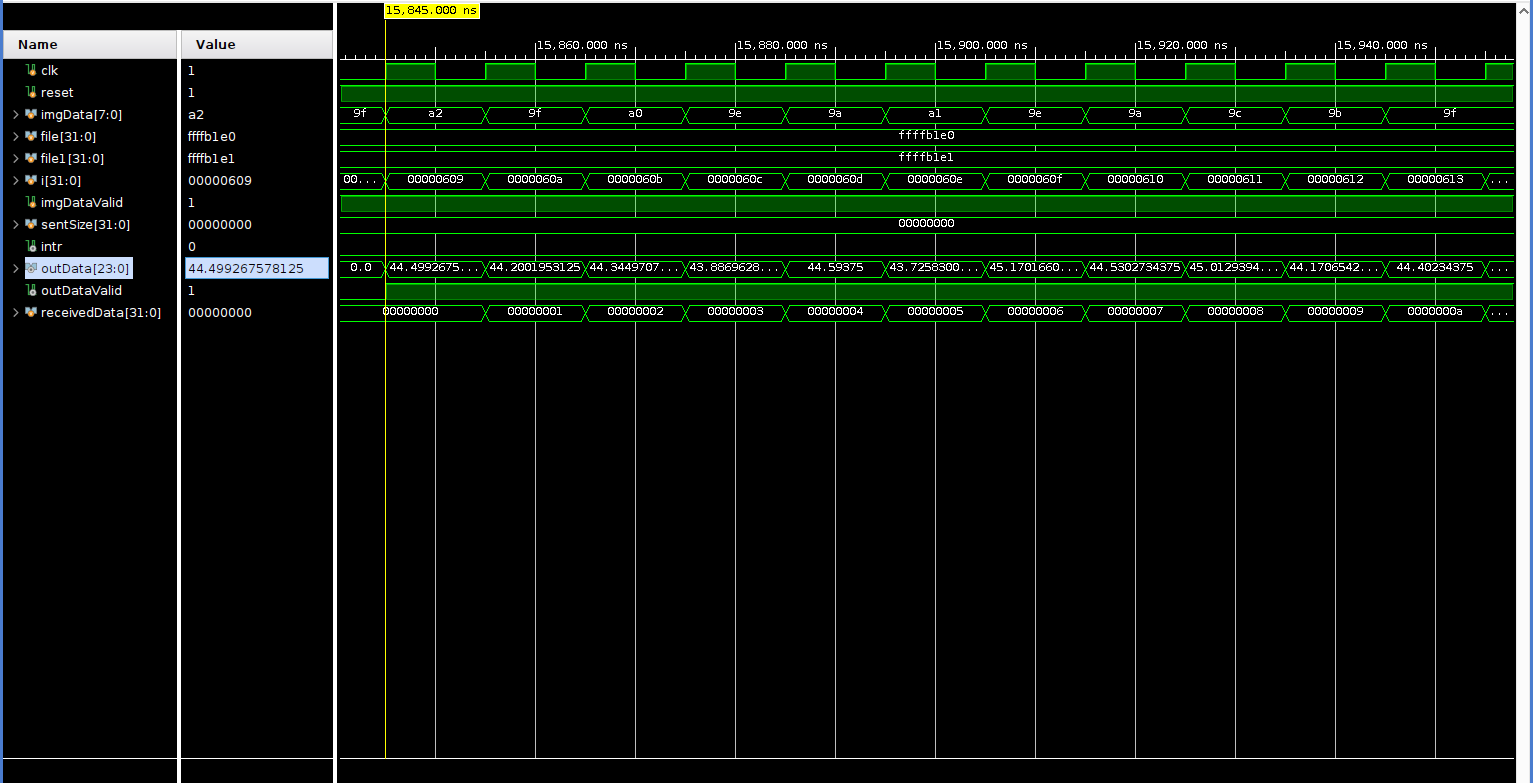
\includegraphics[width=1\linewidth]{images/simulationWaveform.png}
        \caption{Convolution Simulation}
        \label{fig:conv_tb_simulation}
    \end{figure}

    \begin{table}[ht]
    \centering
    \begin{tabular}{|c|c|c|}
        \hline
        \textbf{Input Data Stream} & \textbf{Obtained Output} & \textbf{Decimal} \\
        \hline
        0xA0A0A0A1A09FA0A1A0 & 44.499267578125 & 44.724472 \\
        0xA0A09FA09F9FA1A09E & 44.2001953125 & 44.424690 \\
        0xA09FA19F9FA1A09EA1 & 44.344970703125 & 44.569893 \\
        0x9FA19C9FA19B9EA19C & 43.886962890625 & 44.109791 \\
        0xA19CA1A19BA1A19CA2 & 44.59375 & 44.817875 \\
        0x9CA19F9BA19F9CA29F & 43.725830078125 & 43.949493 \\
        0xA19FA2A19FA3A29FA3 & 45.170166015625 & 45.396538 \\
        0x9FA29F9FA39F9FA39F & 44.5302734375 & 44.755623 \\
        0xA29FA0A39FA0A39FA0 & 45.012939453125 & 45.238426 \\
        0x9FA09E9FA09E9FA09E & 44.170654296875 & 44.394283 \\
        \hline
    \end{tabular}
    \caption{Convolution Operation input data, obtained output, and actual output}
    \label{tab:data_stream}
\end{table}

    \noindent The table \ref{tab:data_stream} shows the set of input and output for one 3x3 pixel data in the first column which is 72 bits wide the second column shows obtained output in its equivalent 16-bit fixed point representation adopted in this project, and the last column shows the expected convolution operation result in decimal. The results shown in the \ref{tab:data_stream} are also observed waveform window during the simulation as shown in the figure \ref{fig:conv_tb_simulation}. The figure shows the golden data for comparison, which is seen on \textit{MATLAB}, the first window shows image pixel data, and the second window shows the convolution operation along with added bias.

    \begin{figure}
        \centering
        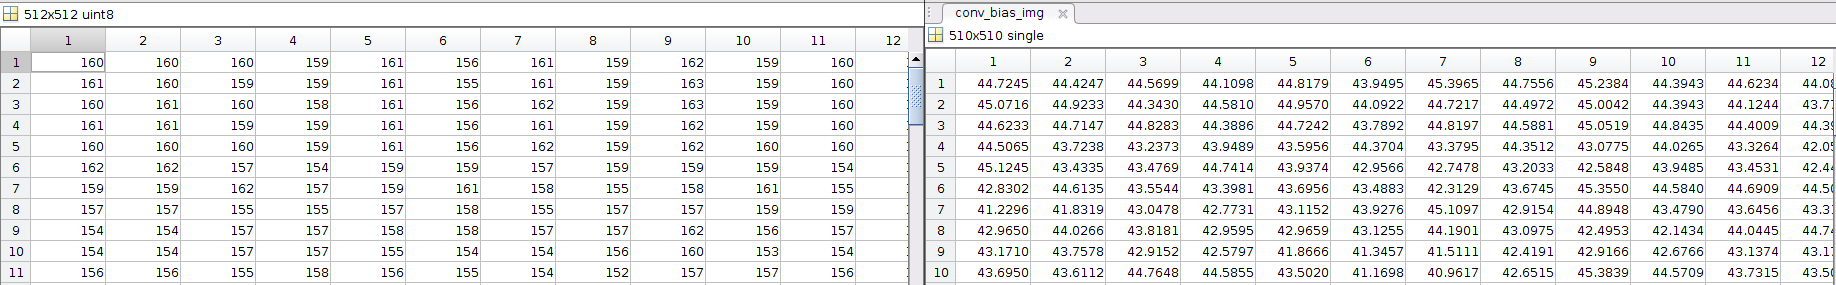
\includegraphics[width=1\textwidth]{images/matlabGoldenData.png}
        \caption{Matlab golden data for Convolution operation}
        \label{fig:matlabGoldenData}
    \end{figure}
    
    \par
    \noindent Now, from the obtained output for a given input, it can be seen that these values are nearly the same when compared to the expected output, the difference is mainly because while adopting a 16-bit fixed point standard from a float32, some precision is lost.

    \subsection{Maxpool Simulation}
    \noindent
    The maxpool logic involves no arithmetic operations and comprises comparison as the only operation thus, whether the maximum value from the appropriate window is obtained is the only point to be verified.
    Figures \ref{fig:convWindow1} and  \ref{fig:convWindow2} represent output convolved data when the convolution kernel is convoluted on the first and the second row. 
    \begin{figure}
        \centering
        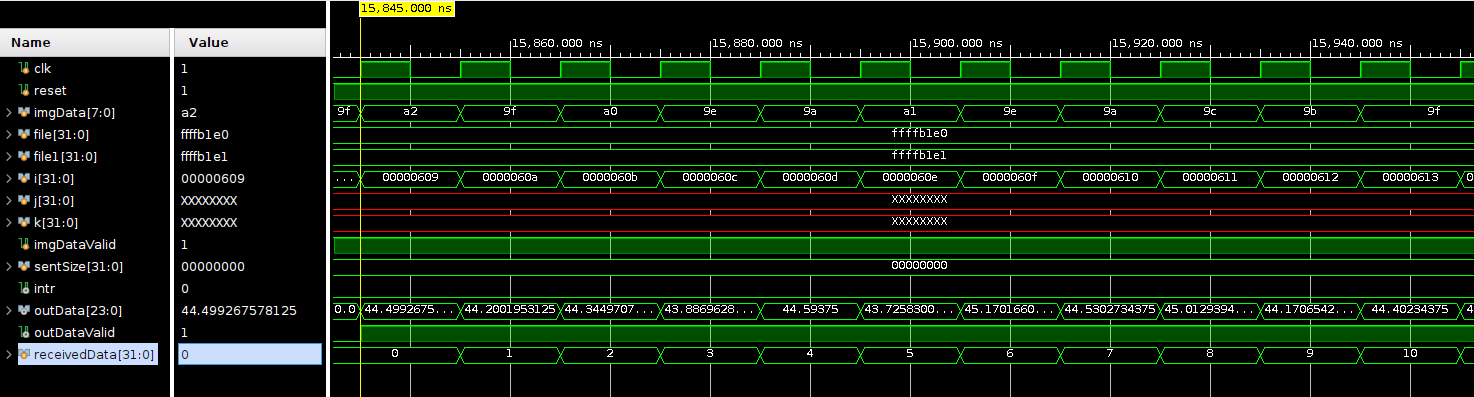
\includegraphics[width=\linewidth]{images/convWindow1.png}
        \caption{Convolution first row output on Vivado Simulator}
        \label{fig:convWindow1}
    \end{figure}
    \begin{figure}
        \centering
        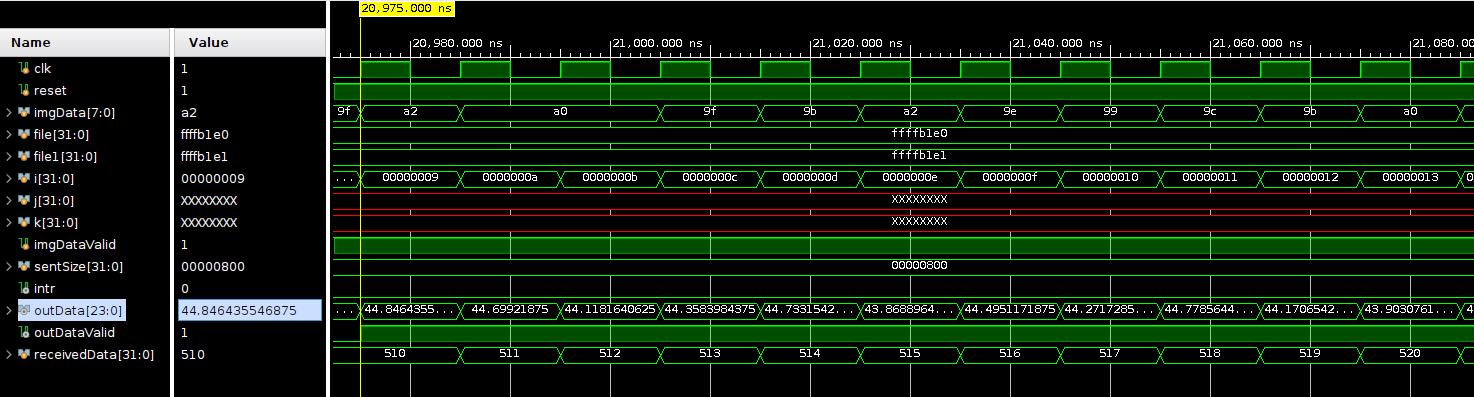
\includegraphics[width=\linewidth]{images/convWindow2.png}
        \caption{Convolution second row output on Vivado Simulator}    
        \label{fig:convWindow2}
    \end{figure}

    \noindent
    Figure \ref{fig:maxpoolrow1} shows the max-pooled output when the kernel is applied on the first two rows(kernel size of 2x2) of convolved data with a stride of 2. For comparison with reference data, figure \ref{fig:matlabMaxpool} shows reference maxpool and convolution data.

    \begin{figure}
        \centering
        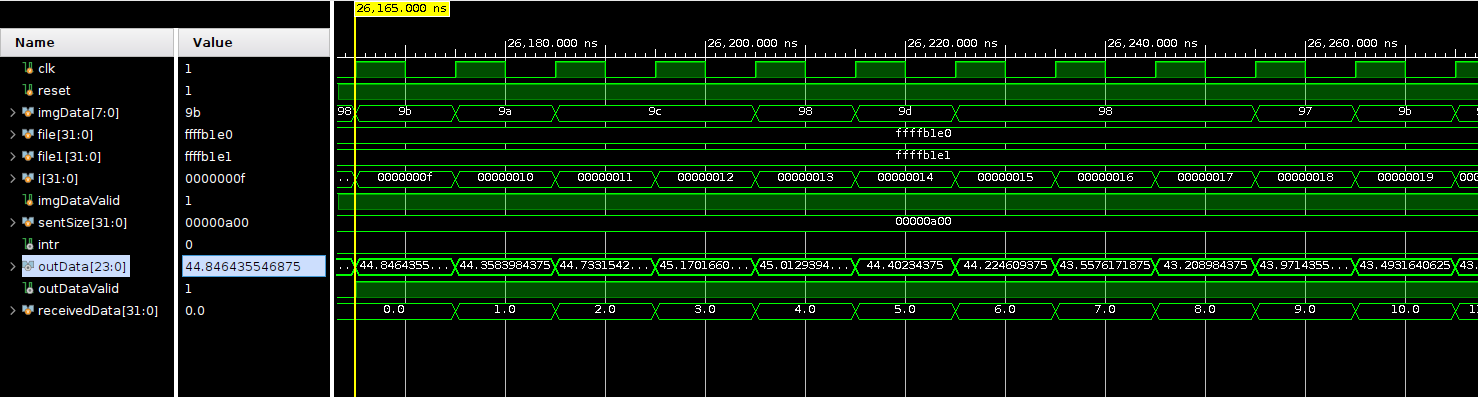
\includegraphics[width=\linewidth]{images/maxpoolRow1.png}
        \caption{Maxpool first row output on Vivado Simulator}
        \label{fig:maxpoolrow1}
    \end{figure}

    \begin{figure}
        \centering
        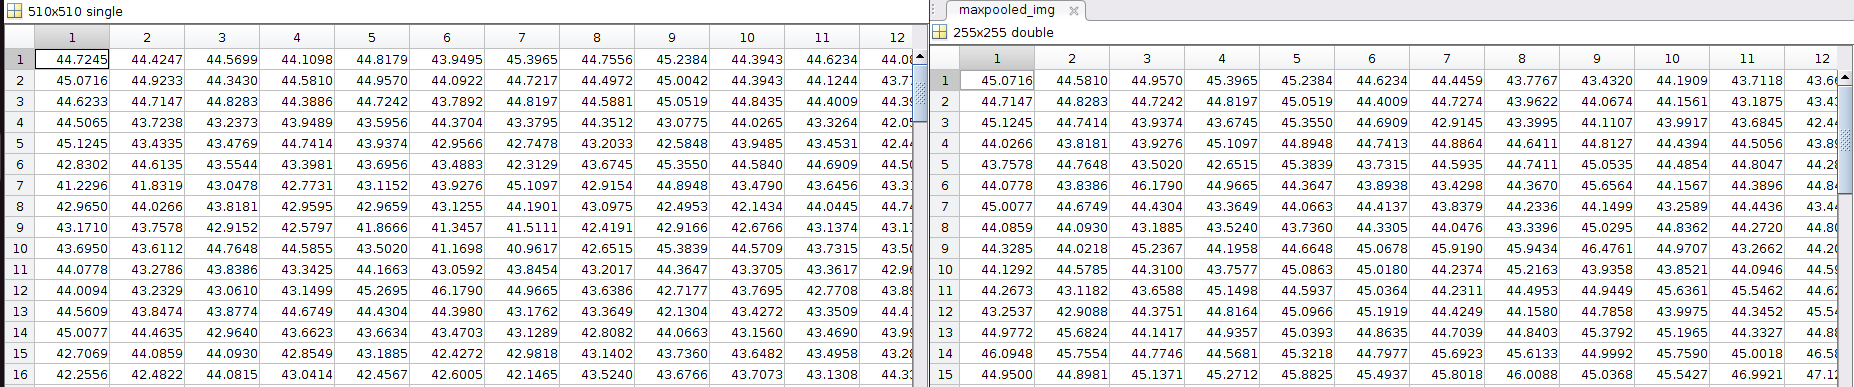
\includegraphics[width=\linewidth]{images/matlabConvMaxRefdata.png}
        \caption{Matlab reference convolution and Maxpool data}
        \label{fig:matlabMaxpool}
    \end{figure}
    
    
    \section{Validation}
    \noindent
    During the initial phase of design and development, it is necessary to evaluate the functionality of the design at the Hardware level, knowing that FPGA-based systems are very critical while implementing on actual hardware. Once the scale of design is increased, it may be difficult to find the bugs and debug the design. Thus, in the initial phase, a hardware-level evaluation is carried out.
    \subsection{Convolution IP Hardware Level Evaluation}
    \noindent
    After the simulation, once the RTL's functionality is verified, the convolution logic is packaged as an IP using the Vivado IP packager tool, and the IP is based on the AXI4 Stream protocol. To receive the image, the PS is programmed to receive the image through the UART interface. The PS is provided with the hardware configuration using an XSA(Xilinx Specification Archive) file. The PS is also programmed to transfer the received image using the DMA to the convolution IP(topConv). A system-level check is performed where the system only performs a convolution operation. The main reason to only perform testing on the Convolution IP is to keep the debug process simple. This acts like an initial testing to check whether, at the hardware level does the data is being received properly by the FPGA through the UART. The system-level block diagram is shown in Figure \ref{fig:block-design}. This design also includes a debug core, which can be seen in the block design by the name \textit{System ILA}, which helps observe the waveforms when the actual evaluation of the logic is performed on the board. The debug core enables observing waveforms at the actual hardware level, and can be seen on Vivado. 

    \begin{figure}[H]
        \centering
        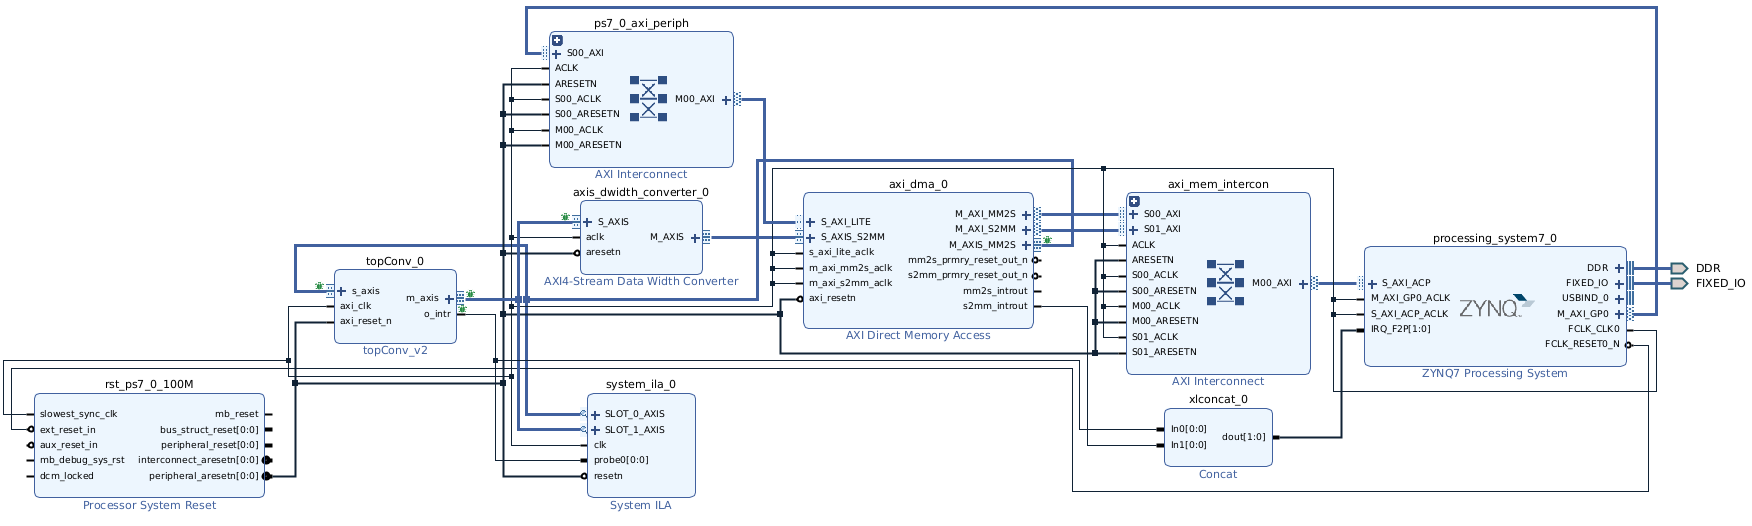
\includegraphics[width=\linewidth]{images/BlockDesign.png}
        \caption{Convolution IP system level block diagram in Vivado}
        \label{fig:block-design}
    \end{figure}
    
    \noindent Steps Involved:
    \begin{enumerate}[noitemsep, topsep=3pt]
        \item Open Hardware Manager in Vivado, connect to the PYNQ-Z2 board
        \item Setup a trigger after which samples are to be collected
        \item Using the Vitis IDE program, the PS 
        \item In Vivado, click on \textit{refresh device} and then program the device
        \item Using Teraterm, set a serial connection between the PC and PYNQ-Z2 
        \item In Vivado, run the trigger 
        \item Using Teraterm, send the image in binary format
        \item Observe waveforms generated from debug cores on Vivado
    \end{enumerate}

    \noindent
    Figures \ref{fig:dmaTrigger} and \ref{fig:convDataTrigger} show the triggers which have been setup, as can be seen in the Trigger setup window appearing at the bottom right corner. The triggers start to sample signals whenever \textit{valid} signal goes low-to-high. Here, triggers have been setup for mainly two tasks:

    \begin{enumerate}[noitemsep, topsep=3pt]
        \item Check whether appropriate Image data is transferred by DMA to the Convolution IP
        \item Check if convoluted data is being transferred from Convolution IP to DMA
    \end{enumerate}

    \begin{figure}[H]
        \centering
        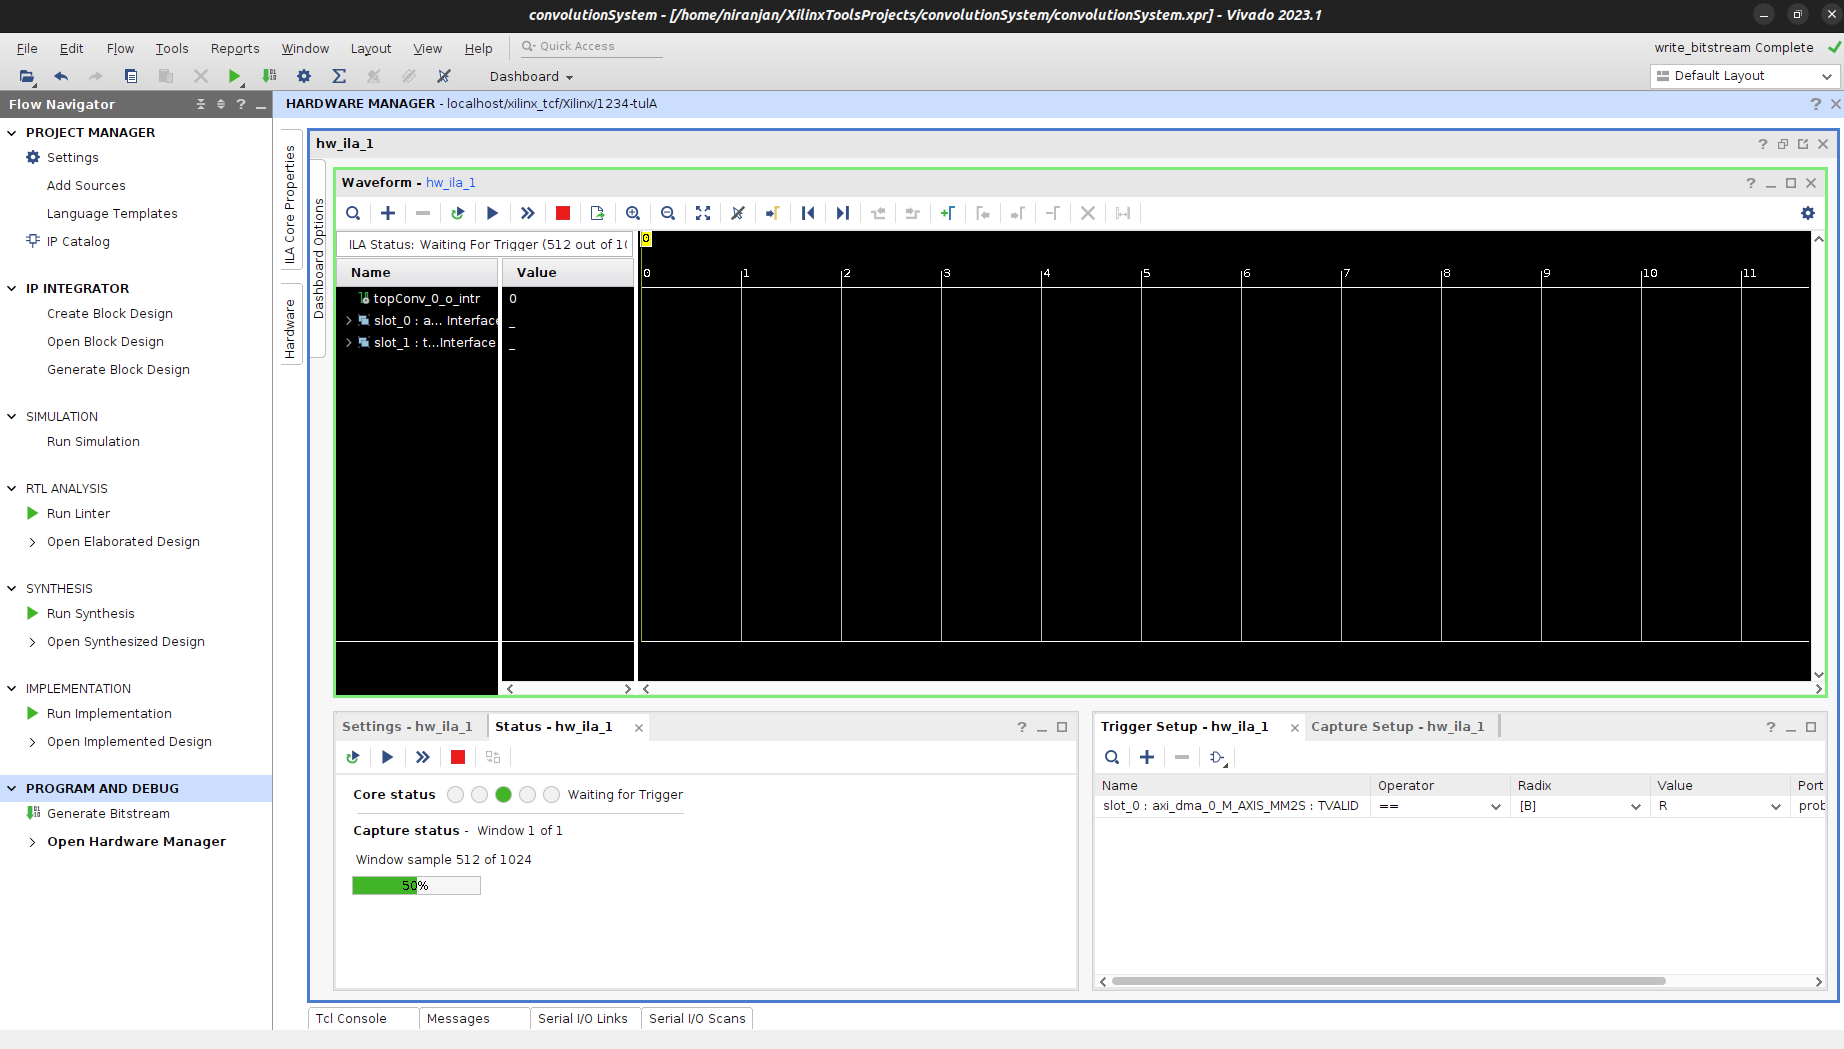
\includegraphics[width=0.87\linewidth]{images/dmaTrigger.png}
        \caption{Debug core waiting for DMA Image Data Valid}
        \label{fig:dmaTrigger}
    \end{figure}

    \begin{figure}[H]
        \centering
        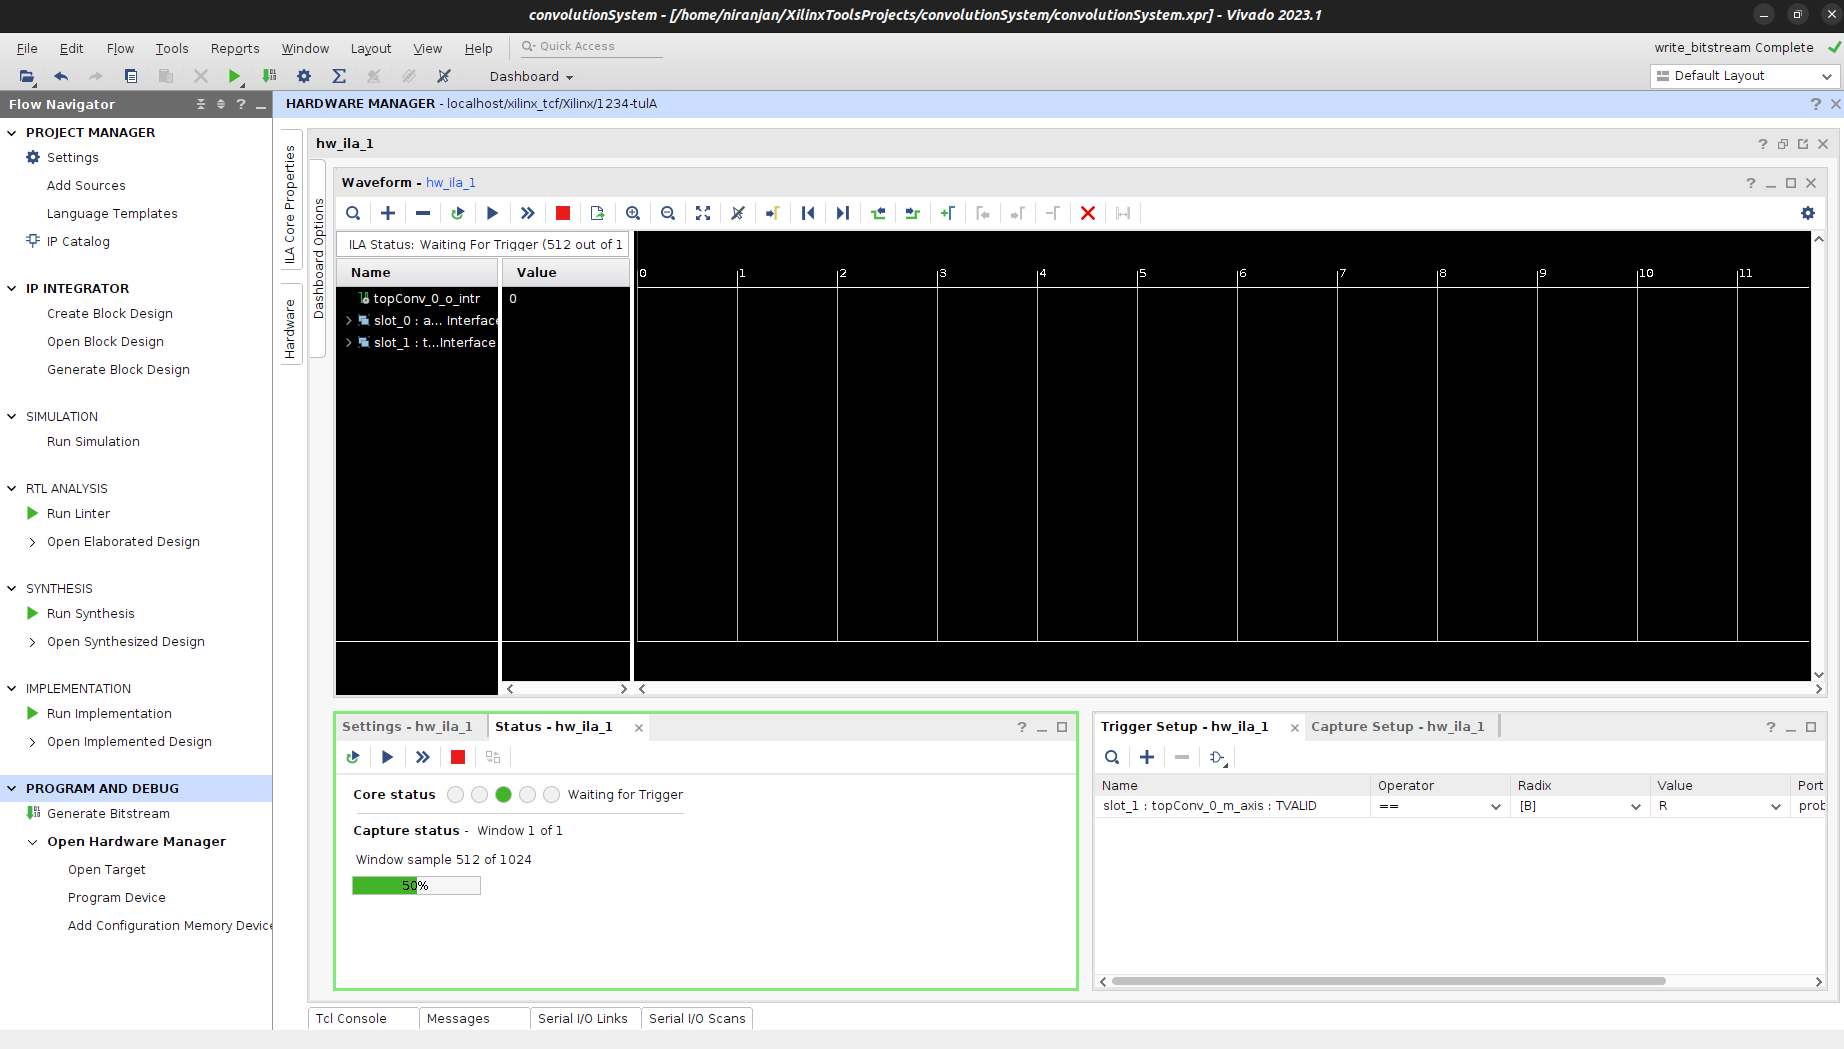
\includegraphics[width=0.87\linewidth]{images/convDataTrigger.png}
        \caption{Debug Core waiting for Convolution IP Output Data Valid}
        \label{fig:convDataTrigger}
    \end{figure}

    \begin{figure}[H]
        \centering
        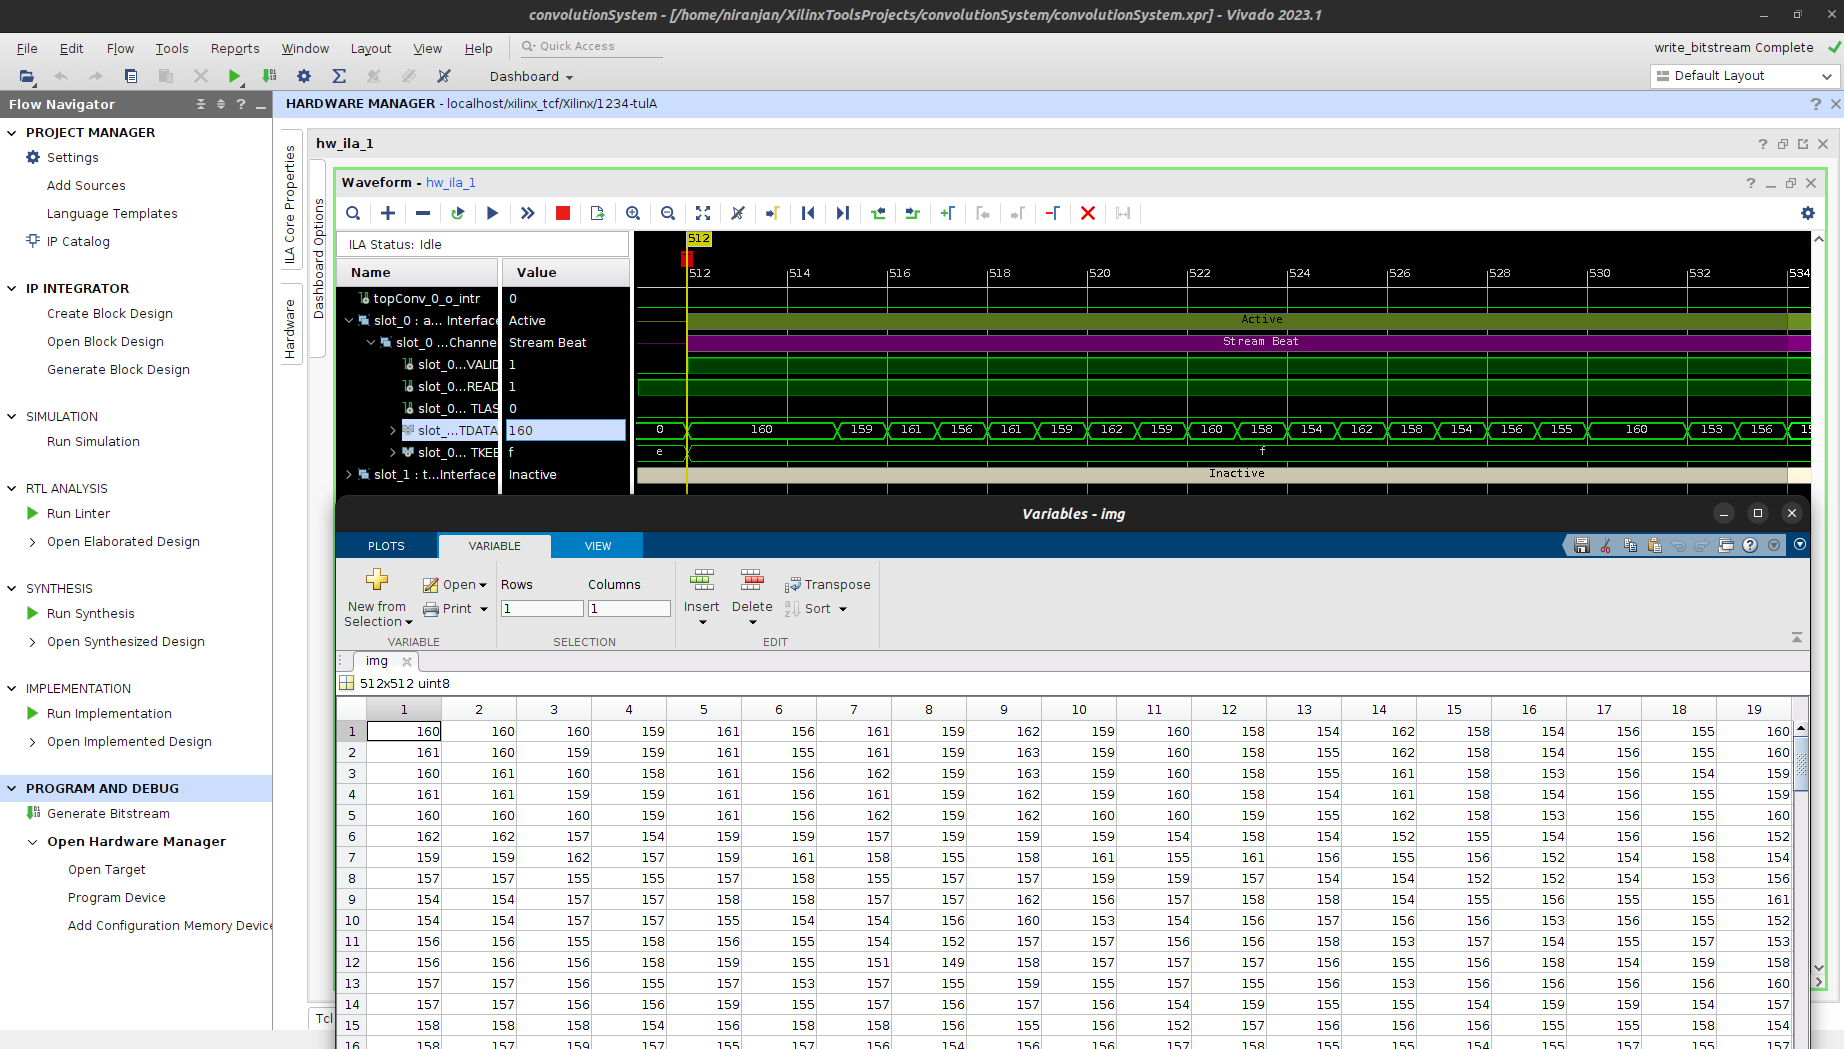
\includegraphics[width=1\linewidth]{images/imageDataTriggered.png}
        \caption{Image Data samples captured after DMA valid signal is triggered}
        \label{fig:imageDataTriggered}
    \end{figure}

    \begin{figure}[H]
        \centering
        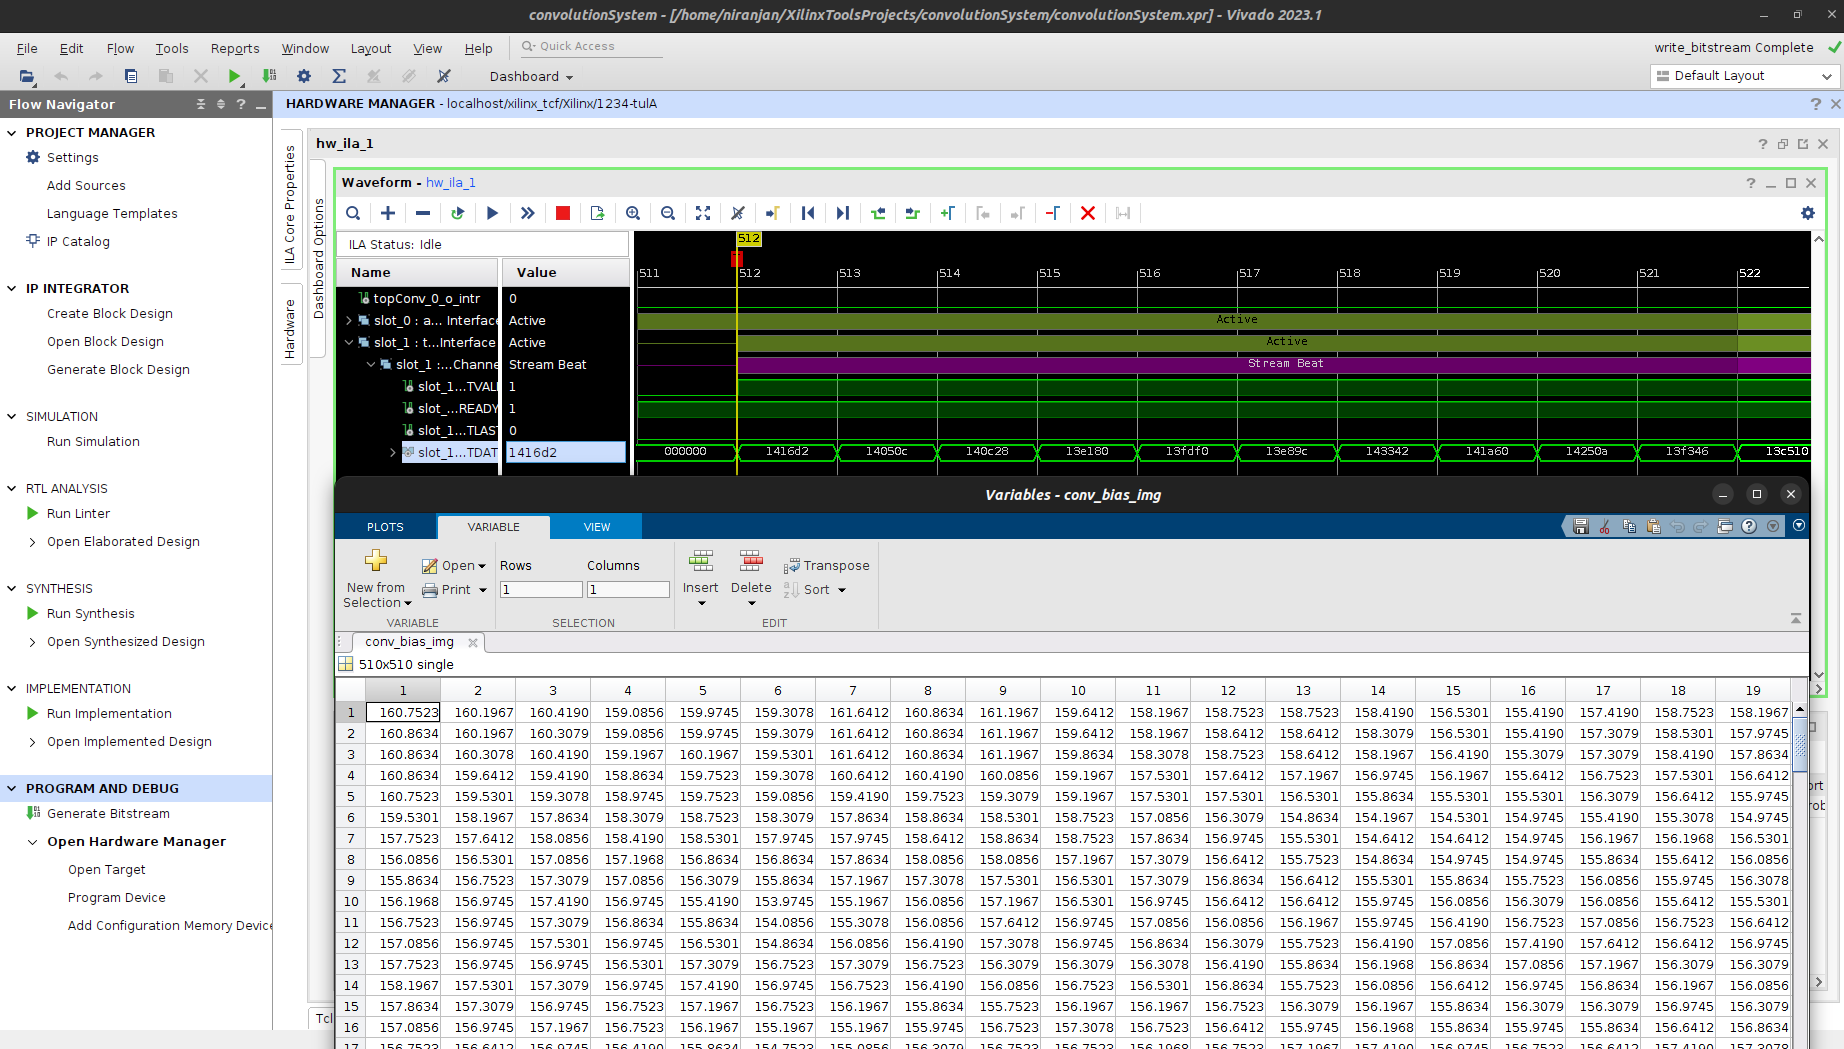
\includegraphics[width=1\linewidth]{images/convResultTriggered.png}
        \caption{Convolution Data samples captured after Convolution IP valid is triggered}
        \label{fig:convResultTriggered}
    \end{figure}

    \noindent
    Figure \ref{fig:imageDataTriggered} shows the captured data after the DMA's valid signal goes low-to-high. The same window contains a MATLAB window, which shows image data in uint8 format. The data captured is the first row of the image, and thus, it can be verified that proper data is being received by the convolution logic module by observing received and actual image pixel data on the waveform and MATLAB window.
    
    \noindent
    Figure \ref{fig:convResultTriggered} shows the output data captured by the debug core when the valid signal of the convolution IP goes from low to high. The data received results from a convolution operation performed on the first three rows for the initial few windows. Table \ref{tab:convDebugWaveform} shows equivalent decimal numbers corresponding to received hexadecimal data and expected convolution output data. The debug window has no option to convert data to a comparable form, thus, conversion is to be performed manually.
    \par \noindent
    The kernel and the bias used for the convolution operation at the hardware level are as follows.
    \begin{center}
    \begin{tabular}{|c|c|c|}
    \hline
    1/9 & 1/9 & 1/9 \\ \hline
    1/9 & 1/9 & 1/9 \\ \hline
    1/9 & 1/9 & 1/9 \\ \hline
    \end{tabular}
    \end{center}

    \[
    \text{bias} = 0.6411843299865723
    \]
    
    \par \noindent
    (Note initially 13 bits were used for fraction bits, but later on it was found that the integer part requires at least 3 bits thus, at a later stage, 12 bits of fraction and 3 bits of integer were adopted.)

    \begin{table}[H]
    \centering
    \renewcommand{\arraystretch}{1.3} % increases row height for better spacing
    \begin{tabular}{|c|c|c|}
    \hline
    \textbf{Convolution Output} & \textbf{Fixed Point Standard} & \textbf{MATLAB Reference} \\
    \textbf{(Hexadecimal)} & \textbf{Equivalent} & \textbf{Data} \\
    \hline
    1416d2 & 160.713134765625 & 160.75230 \\
    14050c & 160.15771484375  & 160.19673 \\
    140c28 & 160.3798828125   & 160.41896 \\
    13e180 & 159.046875        & 159.08563 \\
    13fdf0 & 159.935546875     & 159.97452 \\
    13e89c & 159.26904296875   & 159.30785 \\
    143342 & 161.601806640625  & 161.64117 \\
    141a60 & 160.82421875      & 160.86342 \\
    14250a & 161.157470703125  & 161.19675 \\
    13f246 & 159.571044921875  & 159.64119 \\
    \hline
    \end{tabular}
    \caption{Convolution Outputs Compared with MATLAB Reference Data}
    \label{tab:convDebugWaveform}
    \end{table}

    \noindent
    Thus, the appropriate image data is transferred to the Convolution IP, and the corresponding appropriate convolution output is also obtained. Due to fixed-point representation, the data suffers from loss of precision.

    \newpage
    
    

    

    
 \newpage
\chapter{Results \& Discussion}

    \section{CNN Model}
    \noindent
    The model developed for the deployment has the following parameters at each layer:
    \begin{figure}[H]
        \centering
        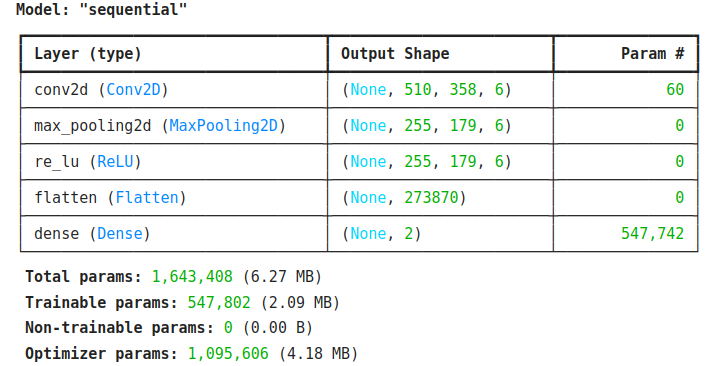
\includegraphics[width=1\linewidth]{images/modelSummary.png}
        \caption{Model Summary}
        \label{fig:enter-label}
    \end{figure}
    The following are the hyperparameters:
    \begin{enumerate}
        \item Number of epochs 15
        \item Activation function ReLU for the convolution layer and Softmax for final probabilities
    \end{enumerate}

    \noindent
    A validation accuracy of 92.22\% is obtained when tested on a validation dataset. The following figures show the Training and Validation accuracy plots and the confusion matrix. It must be noted that all benign cases are accurately predicted. This is specific to the validation dataset for some other set of datasets, this may not be the case.

    \begin{figure}[H]
        \centering
        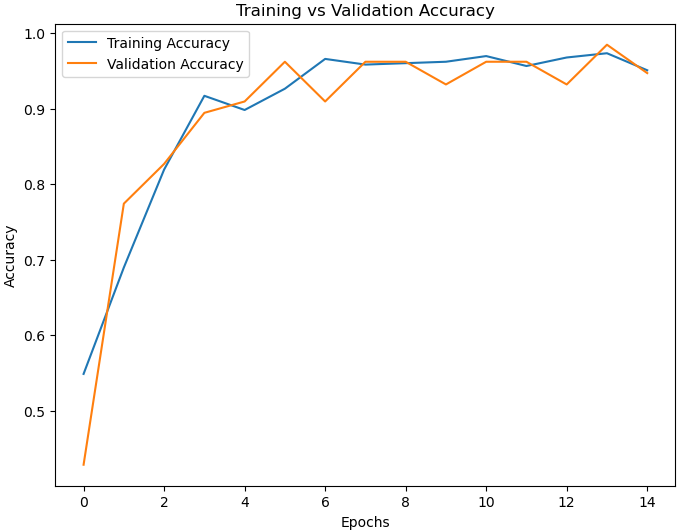
\includegraphics[width=1\linewidth]{images/trainValAcc.png}
        \caption{Train and Validation Accuracy Plot}
        \label{fig:enter-label}
    \end{figure}

    \noindent
    Some of the classification model parameters have been shown below, as per the reports generated in Python from Jupyter:

    \begin{figure}[H]
        \centering
        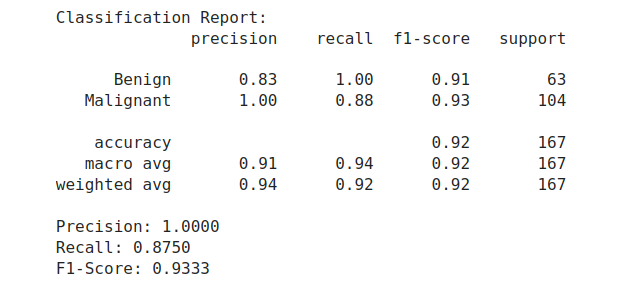
\includegraphics[width=1\linewidth]{images/classificationReport.png}
        \caption{Classification Report for the CNN model}
        \label{fig:enter-label}
    \end{figure}

    \begin{figure}[H]
        \centering
        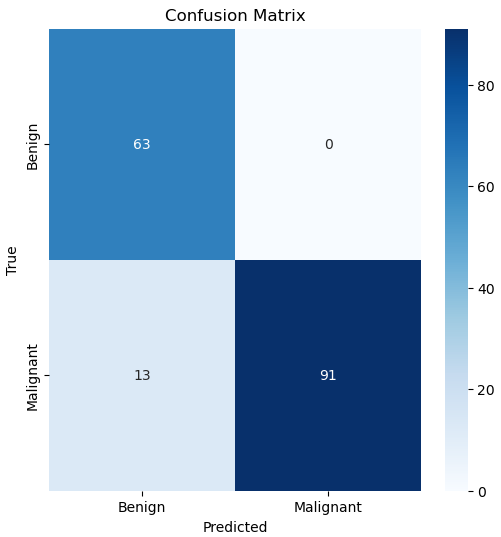
\includegraphics[width=0.75\linewidth]{images/conf_matrix.png}
        \caption{Confusion Matrix evaluated on Validation dataset}
        \label{fig:enter-label}
    \end{figure}
    
    \section{FPGA Experimental Results Analysis}
    \noindent
    The final convolution and max pool logic are evaluated on the hardware, and it is observed and verified that the desired appropriate feature maps are being generated.
    The entire design is implemented on the PYNQ-Z2 FPGA, which belongs to the Xilinx (now AMD) ZYNQ 7000 SoC series. The entire design was evaluated well for the timing performance at 100MHz, but while the final block level design, since the Vivado placer is not well optimized, it led to some routing congestion, and as a result, a slack of 0.105ns was observed, hence the final design works on a frequency slightly less than 100MHz. The table \ref{tab:onchip-resources} shows the resource utilisation report for the design implemented on the PL fabric.

    \begin{table}[h!]
    \centering
    \begin{tabular}{|l|c|c|c|}
        \hline
        \textbf{On-chip resources} & \textbf{Number of resources} & \textbf{Occupied resources} & \textbf{Utilization} \\
        \hline
        LUTs         & 53,200    & 9,529     & 17.9\%   \\
        Flip-Flops   & 106,400   & 7,122     & 6.69\%   \\
        BRAM         & 140       & 128.5     & 91.79\%  \\
        DSP Slices   & 220       & 9         & 4.09\%   \\
        \hline
    \end{tabular}
    \caption{FPGA On-Chip Resource Utilisation}
    \label{tab:onchip-resources}
    \end{table}

    \noindent

    \[
    \text{TPS} = \frac{\text{BITS}}{T}
    \]
    Some performance metrics are discussed in the previous work by Li Li et. al [1]. \par \noindent
    The above formula, TPS, is the throughput, BITS is the number of bits operated in time T. Considering a clock frequency of 100MHz, the proposed system throughput is,

    \[
    \text{TPS} = 360 \times 512 \times 16 \times 100\,\text{MHz} = 294.912\,\text{Gbit/s}
    \]

    \[
    P = \frac{\text{Opt}}{\text{Clk\_num}}
    \]
    Where P stands for computing performance, Clk\_num is the number of required clock cycles to complete operations, and Opt is the number of operations.
    
    \begin{table}[H]
    \centering
    \begin{tabular}{|l|c|}
        \hline
        \textbf{Layer} & \textbf{Number of Operations} \\
        \hline
        Convolution & 360x512x9 \\
        Maxpool     & 358x510x3 \\
        Total       & 2206620   \\
        \hline
    \end{tabular}
    \caption{Layer and Number of Operations}
    \label{tab:layer_operations}
    \end{table}

    \noindent
    As per the simulation results, it is observed that the output feature map is obtained after 1855005 ns and starts at 26175 ns. So the total number of clock cycles required for the operation is (1855005-26175)/10 = 182883 cycles. Thus, the computing performance is 12.066 GOP/s, the power consumption is 1.484W, and the energy efficiency is 8.13 GOP/(s.W).

    \section{Experimental Setup}
    \noindent
    The figure \ref{fig:expSetup} shows the experimental setup, as shown in the image, the PYNQ-Z2 board is connected to the PC through Microusb Port, which is also used as a  UART port and employs a USB to UART bridge for UART interface. The Red LED indicates power status, and the  Green LED is the DONE bit, which is HIGH as seen in the setup.
    
    \begin{figure}[H]
        \centering
        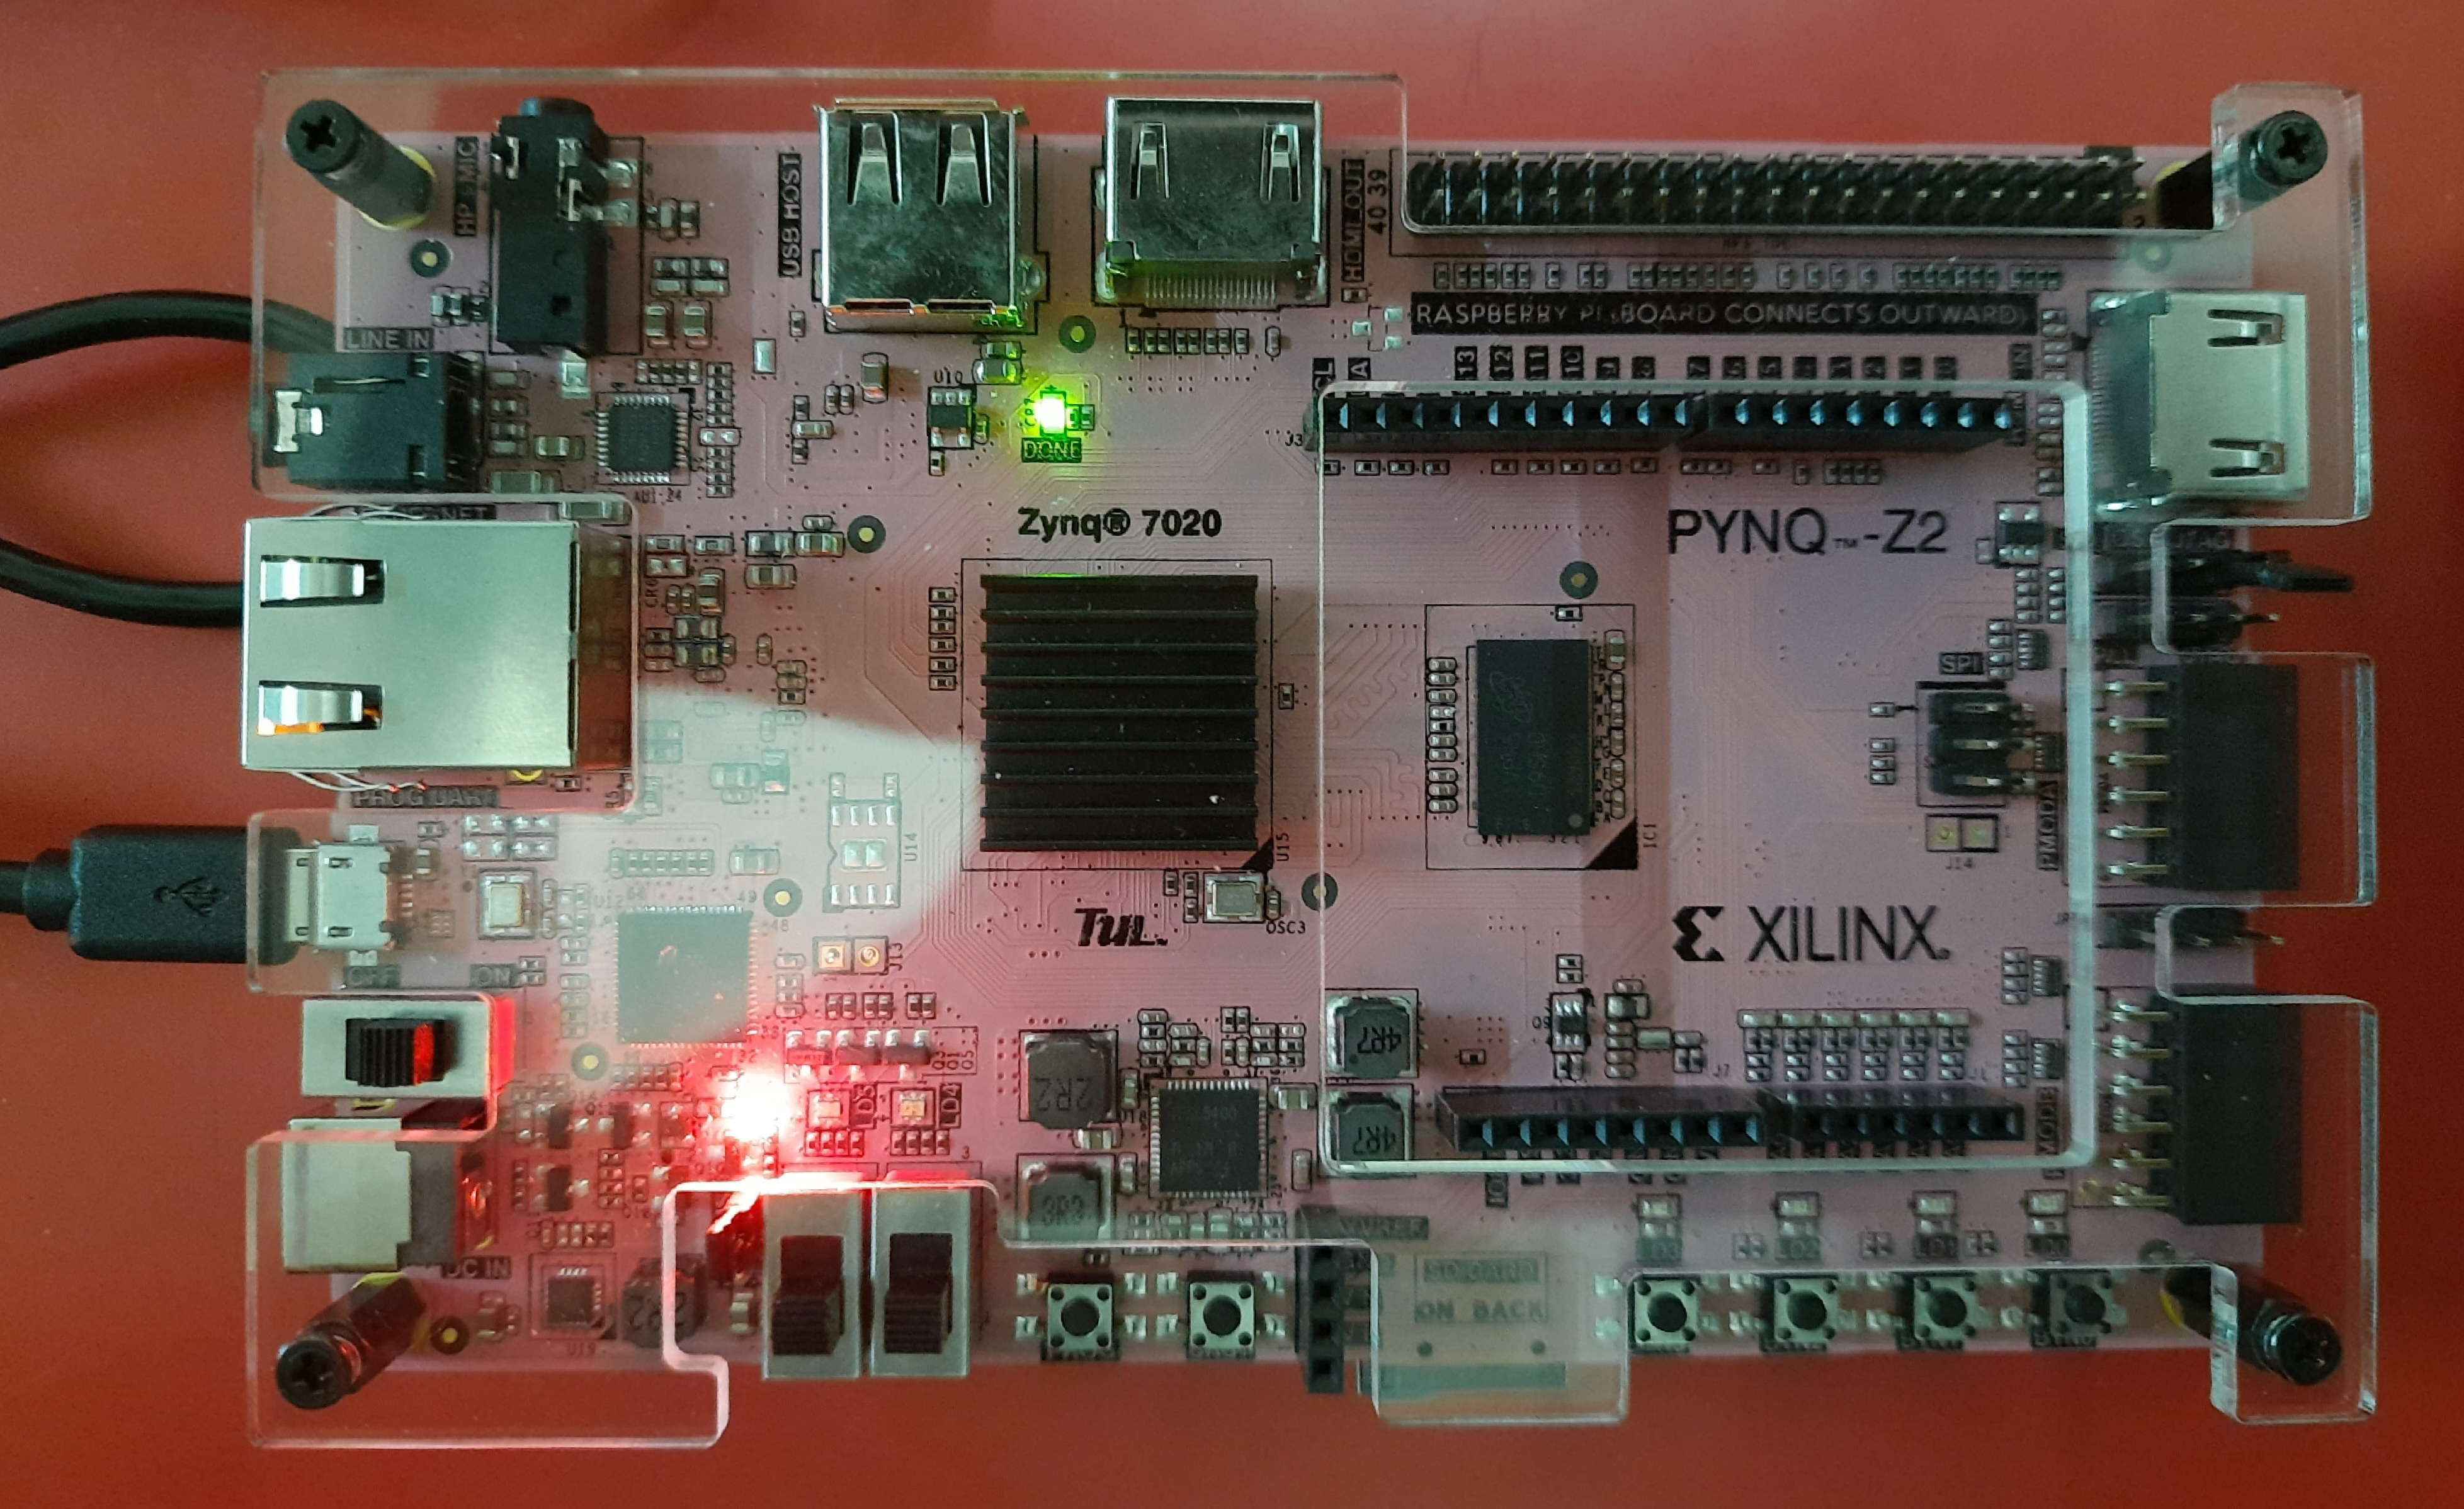
\includegraphics[width=1\linewidth]{images/expSetup.jpg}
        \caption{Experimental Setup}
        \label{fig:expSetup}
    \end{figure}

    \noindent
    A GUI based on Python's Tkinter library transfers the image to the FPGA. It also applies a grayscaling operation and an image resizing operation. Initially, a Serial port must be selected before beginning the image transfer. The figure \ref{fig:gui}  shows the designed GUI with some simple options such as Select Image, Transfer Image, About and EXIT. Also, before the image is transferred, it is shown on the screen.

    \begin{figure}[H]
        \centering
        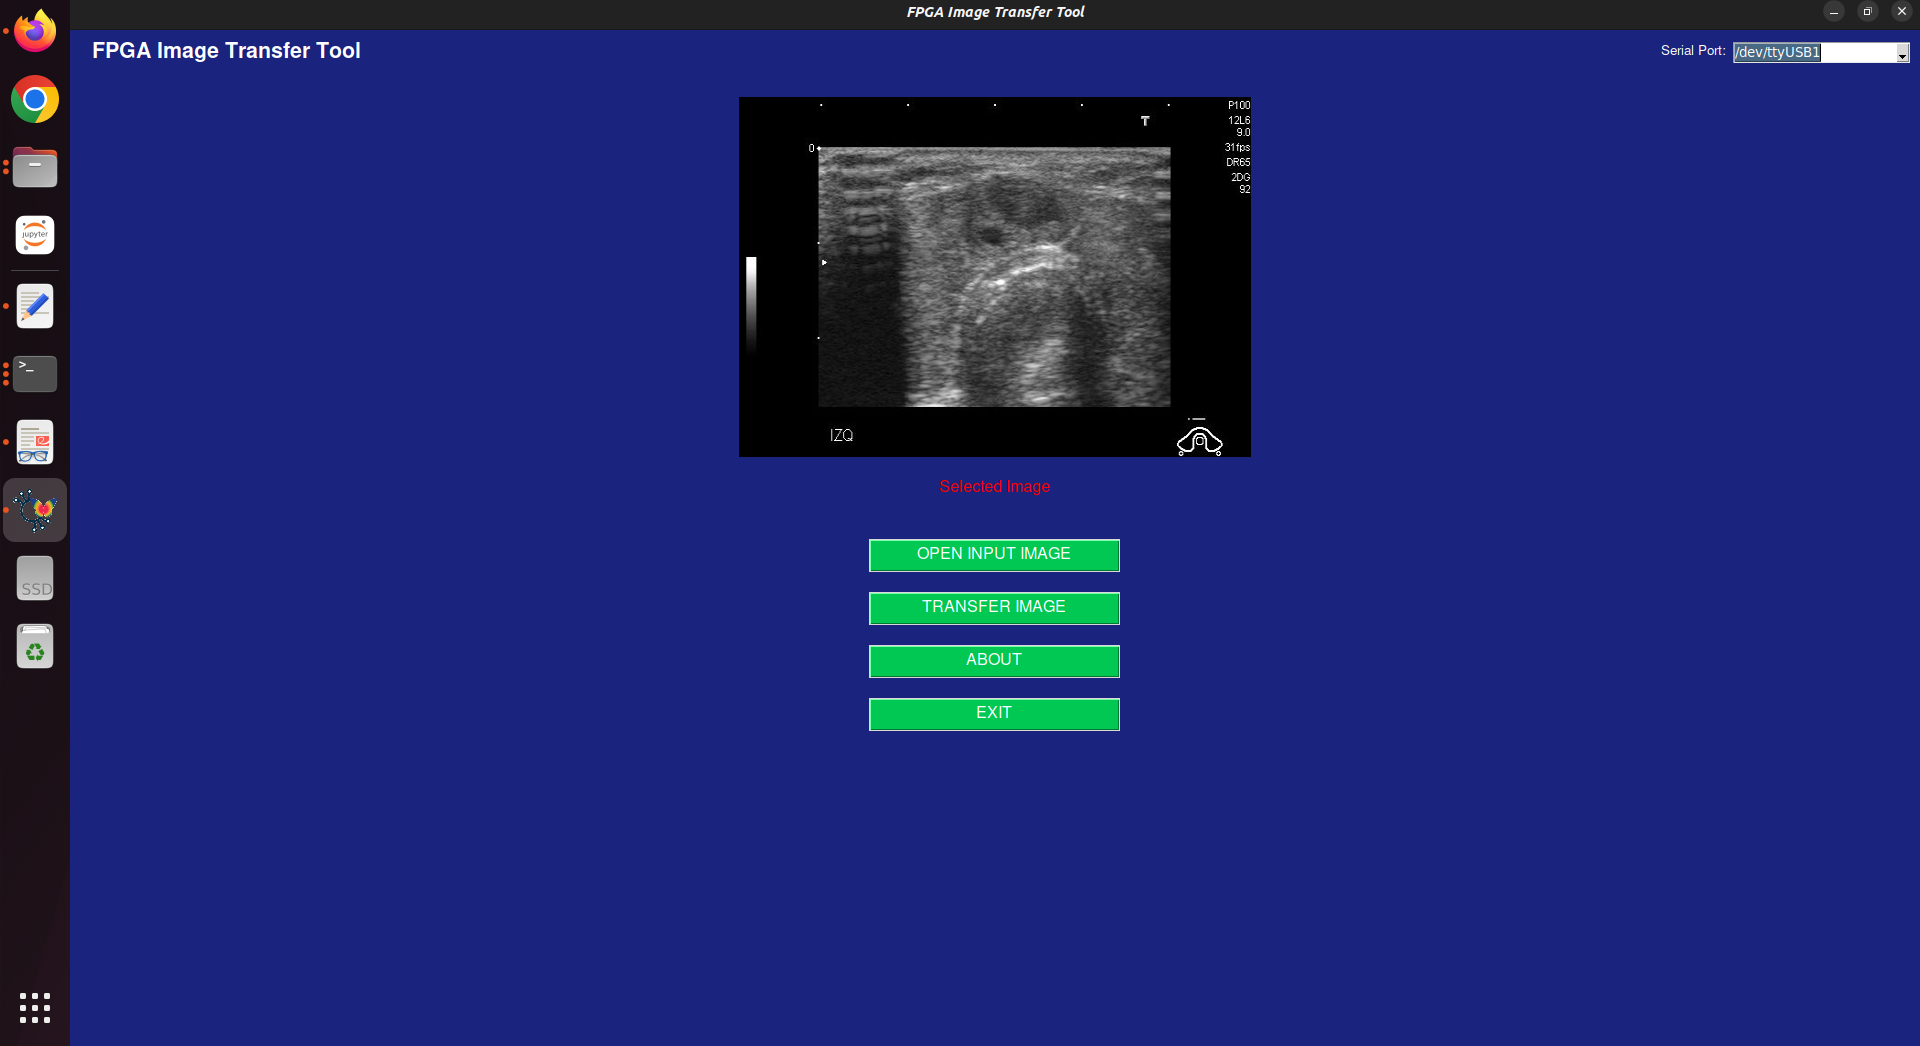
\includegraphics[width=1\linewidth]{images/gui.png}
        \caption{GUI for Image transfer to FPGA}
        \label{fig:gui}
    \end{figure}

    \noindent
    \textbf{Challenges \& Limitations}
    \par \noindent
    The CNN model is very complex, while designing the entire convolution and maxpool acceleration scheme, a lot of data dependencies need to be taken into account. Such a large design needs to be handled properly, ensuring proper architecture-level design since data dependencies need to be taken into account while designing all the compute and data logic. Another critical point is the fact that some of the rules which must be followed come up as a design limitation while designing. The resources and reference guide available for the use of the tools, specifically tutorials available, are very few being able to complete the entire design is a difficult task. The dataset in terms of the number of images available is quite a bit less in amount thus, the model is not that robust.

    

    


    

    

    
     



 \setlength{\parindent}{2em}
\chapter{Conclusion \& Future Scope}
    \section{Conclusion}
    \noindent
    Thus, in this project, an accelerated scheme for Convolution and Maxpool layers has been developed. The interface between Programmable Logic(PL) and Processing System(PS) is achieved through an AXI protocol-based interface using DMA. As discussed earlier, the entire acceleration scheme takes around 1.8ms for the feature map generation due to some design limitations on the design style in the Vivado and Vitis tools, which are used for PL design purposes and PS programming respectively; it was not possible to implement the dense layer which is the final stage in classification. Here, the use of a custom fixed-point standard is used for representing the weights, and thus, the result is a fixed-point (decimal) number it is difficult to take into account the decimal point while developing a logic at the PS level. Based on the proposed acceleration scheme for the convolution pooling architecture, the performance metrics achieved are throughput of 294.912 Gbit/s and a computing performance of 12.066 GOP/s with a power consumption of 1.484W and an energy efficiency of 8.13 GOP/(s.W)

    \section{Future Scope}
    \begin{enumerate}
        \item To develop a robust CNN model along with a fully connected layer 
        \item Develop a data and control logic for intra-convolution and maxpool parallelism architecture
        \item Design a computing scheme for a multiple-layer model 
    \end{enumerate}
    
 \newpage

 \bibliographystyle{plain}
 \begin{thebibliography}{99}

\bibitem{1} L. Li, X. Chen and W. Gao, "Implementation of Convolutional Neural Network Accelerator based on ZYNQ," 2022 IEEE International Conference on Advances in Electrical Engineering and Computer Applications (AEECA), Dalian, China, 2022, pp. 158--165, doi: \texttt{10.1109/AEECA55500.2022.9918905}.

\bibitem{2} J. Shen, Y. Huang, M. Wen and C. Zhang, "Toward an Efficient Deep Pipelined Template-Based Architecture for Accelerating the Entire 2-D and 3-D CNNs on FPGA," \textit{IEEE Transactions on Computer-Aided Design of Integrated Circuits and Systems}, vol. 39, no. 7, pp. 1442--1455, July 2020, doi: \texttt{10.1109/TCAD.2019.2912894}.

\bibitem{3} S. Gowda, T. D, V. B. Sheth, V. R, G. N and H. P, "Thyroid Nodule Detection and Classification Using Deep Learning," 2023 International Conference on Computational Intelligence for Information, Security and Communication Applications (CIISCA), Bengaluru, India, 2023, pp. 200--205, doi: \texttt{10.1109/CIISCA59740.2023.00047}.

\bibitem{4} Y. Habchi, H. Kheddar and Y. Himeur, "Ultrasound Images Classification of Thyroid Cancer using Deep Transfer Learning," 2024 International Conference on Telecommunications and Intelligent Systems (ICTIS), Djelfa, Algeria, 2024, pp. 1--6, doi: \texttt{10.1109/ICTIS62692.2024.10894176}.

\bibitem{5} X. Yang and G. Zhu, "Ultrasound-based discrimination of thyroid cancer based on deep learning," 2024 5th International Conference on Artificial Intelligence and Electromechanical Automation (AIEA), Shenzhen, China, 2024, pp. 939--943, doi: \texttt{10.1109/AIEA62095.2024.10692904}.

\bibitem{6} G. B. Alghanimi, H. K. Aljobouri and K. A. Al-shimmari, "CNN and ResNet50 Model Design for Improved Ultrasound Thyroid Nodules Detection," 2024 ASU International Conference in Emerging Technologies for Sustainability and Intelligent Systems (ICETSIS), Manama, Bahrain, 2024, pp. 1000--1004, doi: \texttt{10.1109/ICETSIS61505.2024.10459588}.

\bibitem{7} P. Qin, K. Wu, Y. Hu, J. Zeng and X. Chai, "Diagnosis of Benign and Malignant Thyroid Nodules Using Combined Conventional Ultrasound and Ultrasound Elasticity Imaging," \textit{IEEE Journal of Biomedical and Health Informatics}, vol. 24, no. 4, pp. 1028--1036, April 2020, doi: \texttt{10.1109/JBHI.2019.2950994}.

\bibitem{8} N. Veni, M. Harshavardhan, L. T K, P. Sritha, P. Chitra and H. Yaseen, "Automatic Detection of Thyroid Nodules in Ultrasound Images using Convolutional Neural Networks for Early Cancer Diagnosis," 2024 International Conference on Artificial Intelligence and Quantum Computation-Based Sensor Application (ICAIQSA), Nagpur, India, 2024, pp. 1--6, doi: \texttt{10.1109/ICAIQSA64000.2024.10882379}.

\bibitem{9} T. K. Devi, K. N. Baluprithviraj, J. S. Suresh, G. Kalaiarasi, A. S. Sagayaraj and P. Sakthivel, "Detection and Characterization of Thyroid Cancer Nodule Using Deep Neural Networks -A Review," 2024 15th International Conference on Computing Communication and Networking Technologies (ICCCNT), Kamand, India, 2024, pp. 1--6, doi: \texttt{10.1109/ICCCNT61001.2024.10723941}.

\bibitem{10} M. Bal-Ghaoui, M. H. E. Y. Alaoui, A. Jilbab and A. Bourouhou, "Approaching Cross-Disease Features for Improved Classification of Thyroid and Breast Cancer in Ultrasound Images," 2023 3rd International Conference on Innovative Research in Applied Science, Engineering and Technology (IRASET), Mohammedia, Morocco, 2023, pp. 1--5, doi: \texttt{10.1109/IRASET57153.2023.10153008}.

\bibitem{11} A. Umamaheswari, S. Kripa and V. Jeyalakshmi, "Realization of CNN Using Hybrid Multiplier With PYNQ-Z2," 2024 15th International Conference on Computing Communication and Networking Technologies (ICCCNT), Kamand, India, 2024, pp. 1--7, doi: \texttt{10.1109/ICCCNT61001.2024.10725453}.

\bibitem{12} R. M. R. Yanamala and M. Pullakandam, "An Efficient Configurable Hardware Accelerator Design for CNN on Low Memory 32-Bit Edge Device," 2022 IEEE International Symposium on Smart Electronic Systems (iSES), Warangal, India, 2022, pp. 112--117, doi: \texttt{10.1109/iSES54909.2022.00033}.

\bibitem{13} J. W. Cui, Y. S. Zhou, F. Zhang, C. Yin and D. L. Xiang, "FPGA implementation of convolutional neural network based on pipeline architecture," \textit{Journal of Beijing University of Chemical Technology (Natural Science Edition)}, vol. 48, no. 5, pp. 111--118, 2021, doi: \texttt{10.13543/j.bhxbzr.2021.05.014}.

\bibitem{14} Gong Jie, Zhao Shuo, He Hu and Deng Ning, "Design of Quantized CNN Acceleration System Based on FPGA," \textit{Computer Engineering}, vol. 48, no. 3, pp. 170--174+196, 2022, doi: \texttt{10.19678/j.issn.1000-3428.0060675}.

\end{thebibliography}

\end{document}
